\chapter{多元函数微分}
\label{chap:multivariate-calculus}
\label{chap:multivariable-functions}

当输入由一个实数变成多个坐标时，函数可以沿不同方向变化。逐个坐标观察能否描述整体变化？本章从联合极限和偏导数出发，用线性近似回答这个问题；再把输出和自变量扩展到向量与矩阵，研究高阶变化和由方程确定的局部关系。

本章使用第~\ref{chap:linear-operations}章的向量和矩阵运算、第~\ref{chap:linear-representation}章的线性映射、第~\ref{chap:linear-analysis}章的特征值，以及第~\ref{chap:limits-continuity}章的极限和第~\ref{chap:univariate-differentiation}章的一元微分。微分描述局部变化；下一章将研究多维区域、路径和曲面上的累计。

\par\Needspace{14\baselineskip}

\label{sec:analysis-multivariable-differentiation}
\label{sec:multivariable-differentiation}

一元微分研究输入改变一点时输出随之改变多少：导数$f'(a)$是输出改变量与输入改变量之比的极限。许多量却同时依赖多个输入，例如平板上一点的温度由横、纵两个坐标决定，模型的损失由成千上万个参数决定。

以$f(x,y)=x^2+xy+y^2$为例，输入是平面上的点$(x,y)$，输出是一个实数。把$z=f(x,y)$想成地形的高度、$(x,y)$想成地图上的位置，“输入改变一点”就有无穷多种方式：只向东走、只向北走、斜着走，或者沿一条弯曲的路线靠近。本章回答两个问题：能否用有限个数同时描述所有这些走法下的输出变化；这种描述在什么条件下可靠。

本章先把一元的极限与连续推广到多个坐标同时趋近的情形，再沿坐标轴和固定方向求变化率，得到偏导数、梯度和方向导数。然后要求一个线性函数同时近似所有走法下的变化，这就是可微性；梯度由此可以解释为最快上升的方向。高阶微分用Hessian矩阵描述曲面的弯曲，并据此判别极值。

此后让输出也变成多个实数，即向量值函数，它的线性近似由Jacobian矩阵表示；参数排成矩阵时，按矩阵形状书写同样的线性近似，并用它分析扰动及近似误差。最后把问题反过来：给定一组方程，能否在一点附近把一部分变量解成其余变量的函数，这就是隐函数与反函数定理。
全章中，梯度只描述标量输出，Jacobian矩阵记录多个输出分量的变化，两者的形状与用途不混用。

向量、矩阵、迹与行列式沿用第~\ref{chap:linear-operations}章，线性映射沿用第~\ref{chap:linear-representation}章，特征值沿用第~\ref{chap:linear-analysis}章；极限、距离与连续沿用第~\ref{chap:limits-continuity}章，微分沿用第~\ref{chap:univariate-differentiation}章的结论，本章的微分计算不使用积分极限定理，区域积分的条件在后续各节说明。
偏导数与局部线性近似可参考\scite{math-openstax-calculus3}，严格的多元微分论证可参考\scite{math-lebl2026analysis2}。

\section{多元标量函数的极限和连续性}
\label{sec:multivariable-limits-continuity}

本节研究定义在$D\subseteq\mathbb R^d$上的实值函数$f:D\to\mathbb R$。一元时，$x\to a$只能从左右两侧靠近；在平面上，点可以从任意方向、沿任意曲线靠近基点，极限与连续性的定义必须同时控制所有这些靠近方式。为此，输入的接近程度改用欧氏距离度量，输出误差仍用实数的绝对值度量。

\subsection{多元函数与联合极限}

本节的基本对象在每个输入点给出一个实数。$d=2$时这类函数最容易画出来：把$f(x,y)$当作水平位置$(x,y)$上方的高度，所有点$(x,y,f(x,y))$组成一张曲面，称为函数的图像。
\begin{definition}[多元标量函数]
\label{def:multivariable-scalar-function}
设$d$为正整数、$D\subseteq\mathbb R^d$。映射$f:D\to\mathbb R$称为多元标量函数；它把整个输入点$\bm x=(x_1,\ldots,x_d)^\top$映为一个实数$f(\bm x)$。
\end{definition}
例如$f(x,y)=x^2+xy+y^2$在$(1,2)$处取值$1+2+4=7$。观察这类函数常用两种办法。
第一种是切片：固定$y=2$，得到一元函数$x\mapsto x^2+2x+4$。几何上，这是用竖直平面$y=2$去截曲面，截出一条曲线；它只反映原函数在一条直线上的取值。
第二种是等值曲线：把函数值相同的点连起来。例如$x^2+xy+y^2=7$是平面上一个经过$(1,2)$的倾斜椭圆，就像地图上的等高线。

后文的偏导数就是切片曲线的斜率，梯度则与等值曲线的方向有关。在此之前，极限与连续性要说明：不限于某条切片、在整个平面中趋近基点时，函数值怎样变化。

\paragraph{联合极限的判别}

在平面中，输入可以沿直线、抛物线、螺旋线等路径趋近基点。极限的定义要用一个条件同时控制所有允许的输入，不能按路径分别选择误差范围；做法是只看输入到基点的距离。
\paragraph{极限的定义}
\label{sec:multivariable-joint-limits}

一元极限中，条件$0<|x-a|<\delta$表示$x$落在$a$两侧、半径为$\delta$的小区间内且不等于$a$。在平面上，与之对应的是以$\bm a$为圆心、半径为$\delta$的圆盘去掉圆心；在$\mathbb R^d$中则是去心的球。
欧氏距离$\lVert\bm x-\bm a\rVert_2$同时控制各坐标的偏移，用它代替$|x-a|$，就能把一元极限的邻域条件推广过来。
设$D\subseteq\mathbb R^d$，$f:D\to\mathbb R$，$\bm a$是$D$的聚点，即以$\bm a$为心的任意小球内都有不同于$\bm a$的定义域点；这保证“$\bm x$在定义域内趋近$\bm a$”确实可以发生。
\begin{definition}[多元函数的极限]
\label{def:multivariable-limit}
若对每个$\varepsilon>0$，都存在$\delta>0$，使得
\[
 \bm x\in D,\quad 0<\lVert\bm x-\bm a\rVert_2<\delta
 \quad\Longrightarrow\quad |f(\bm x)-L|<\varepsilon,
\]
则称$f$在$\bm x\to\bm a$时的极限为$L$，记为$\lim_{\bm x\to\bm a}f(\bm x)=L$。
\end{definition}
定义中的$\delta$只依赖$\varepsilon$（以及固定的$f$与$\bm a$），不依赖输入从哪个方向来。只要点进入半径为$\delta$的去心球，不论它沿直线、沿曲线还是来回跳动地进入，函数值都必须落在$L$的$\varepsilon$范围内。各坐标可以按不同速度趋近，行进方向也可以随位置改变，这些情形都由同一个$\delta$覆盖。

\paragraph{序列判据与路径检验}
与一元情形一样，$\lim_{\bm x\to\bm a}f(\bm x)=L$当且仅当：任意满足$\bm x_n\in D\setminus\{\bm a\}$、$\bm x_n\to\bm a$的序列都有$f(\bm x_n)\to L$。
证明只需把一元序列判据中的$|x_n-a|$换成$\lVert\bm x_n-\bm a\rVert_2$。

沿一条路径趋近基点时取出的点列只是这类序列的特例，由此得到路径检验的两面。

若沿两条路径得到不同的输出极限，就有两个序列的函数值趋于不同的数，极限不存在。反过来，只验证有限条路径，甚至验证全部过基点的直线，都没有覆盖全部序列，不能据此断定极限存在。
先看第一种情形：两条直线就足以否定联合极限。
\begin{example}[沿不同直线得到不同极限]
\label{ex:multivariable-path-limits}
令$f(0,0)=0$，非原点处令$f(x,y)=xy/(x^2+y^2)$。
沿直线$y=kx$（$x\neq0$）代入，得到
\[
 f(x,kx)=\frac{kx^2}{x^2+k^2x^2}=\frac{k}{1+k^2}.
\]
这个值不随$x$变化，却随斜率$k$变化：沿$x$轴（$k=0$）为$0$，沿$y=x$为$1/2$，沿$y=-x$为$-1/2$；沿$y$轴同样为$0$。
所以$f$的值只取决于点所在的方向，不取决于离原点多远。原点附近再小的圆盘里，$f$仍然取遍$-1/2$到$1/2$之间的值，原点处没有联合极限。

另一方面，固定$y=c$时，$x\mapsto f(x,c)$在$c\neq0$时是分母不为零的有理函数，在$c=0$时恒为$0$，都是连续的；固定$x$同理。于是$f$的每条坐标切片都连续，$f$却在原点不联合连续。
\end{example}

第二种情形更隐蔽：所有直线给出相同的极限，联合极限仍可能不存在。
\begin{example}[所有直线极限相同而联合极限不存在]
\label{ex:multivariable-parabola-path-limit}
令$g(0,0)=0$，并在非原点处令
\[
 g(x,y)=\frac{x^2y}{x^4+y^2}.
\]
沿$y=kx$，当$k\neq0$时$g(x,kx)=kx/(x^2+k^2)\to0$；
当$k=0$或沿竖直轴时，函数恒为$0$。所有直线给出的极限都是$0$。
可是沿抛物线$y=x^2$，$g(x,x^2)=x^4/(2x^4)=1/2$。更一般地，沿$y=cx^2$代入得到常数$c/(1+c^2)$，因此原点处没有联合极限。

直线检验失败的原因如下。对$x\neq0$，直线$y=kx$可以写成$y=(k/x)x^2$，相当于取$c=k/x$；靠近原点时$c\to\infty$，函数值$c/(1+c^2)\to0$。函数值为$1/2$的“山脊”沿抛物线$y=x^2$弯进原点，每条固定直线最终都离开山脊，进入函数值很小的区域。
\end{example}

因此路径检验只能否定联合极限；要证明联合极限存在，需要像示例~\ref{ex:multivariable-distance-bound-limit}那样，给出对所有路径同时有效的误差估计。
图~\ref{fig:analysis-process-joint-limit-paths}把直线路径和弯曲路径放到同一函数上，显示只检查直线可能遗漏的趋近方式。
\begin{figure*}[!htbp]
 \centering
 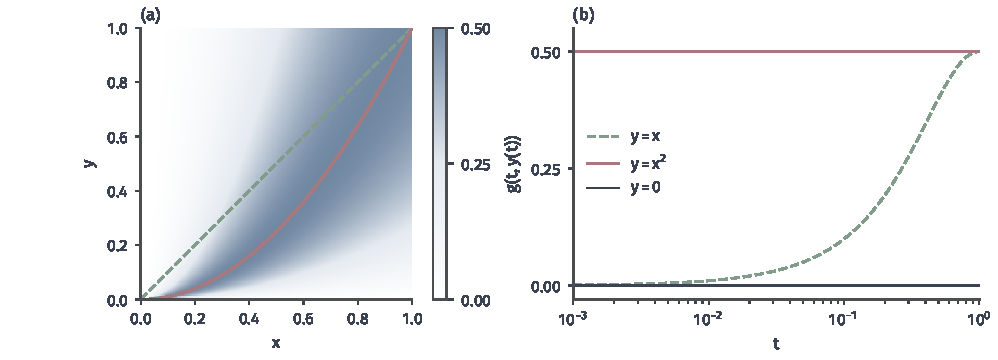
\includegraphics[width=169.0mm]{figures/00-shared/mathematical-preliminaries-upper/00-shared/matplotlib/chapter3-concept-processes/joint-limit-paths.pdf}
 \caption{取前例$g(x,y)=x^2y/(x^4+y^2)$，原点另置零。(a) 第一象限的函数值及三条路径，色阶固定为$0$至$1/2$。(b) 沿$y=0$、$y=x$分别趋零，沿$y=x^2$恒为$1/2$；横轴为正参数$t$的对数刻度，向左趋近原点。不同路径极限足以否定联合极限，有限条路径不能反向证明存在。}
 \label{fig:analysis-process-joint-limit-paths}
\end{figure*}

\paragraph{累次极限与联合极限}
另一种常见做法是逐个坐标取极限，即累次极限。它改变了问题的量词：先令$y\to0$、再令$x\to0$，考察的是
$\lim_{x\to0}\lim_{y\to0}f(x,y)$。内层固定$x\neq0$，让$y$单独趋于$0$；得到一个关于$x$的函数后，外层再让$x$趋于$0$。整个过程没有要求两个坐标同时趋近。
对示例~\ref{ex:multivariable-path-limits}中的$f$，固定$x\neq0$时$f(x,y)\to0$，再令$x\to0$仍为$0$；交换次序同样得到$0$。两个次序的累次极限都为$0$，联合极限却不存在。

累次极限的次序本身也会影响结果。
\begin{example}[两个次序的累次极限不相等]
\label{ex:multivariable-iterated-limits-differ}
在非原点处令$h(x,y)=x^2/(x^2+y^2)$。固定$x\neq0$而令$y\to0$，得到$x^2/x^2=1$；固定$y\neq0$而令$x\to0$，得到$0$。再取外层极限，
\[
 \begin{gathered}
\lim_{x\to0}\lim_{y\to0}h(x,y)=1\\
\lim_{y\to0}\lim_{x\to0}h(x,y)=0.
 \end{gathered}
\]
内层先把一个坐标压到零，相当于先走到某条坐标轴附近，再沿坐标轴靠近原点。$h$在$x$轴上恒为$1$、在$y$轴上恒为$0$，两种次序因而给出不同结果。
\end{example}

所以累次极限相等不是联合极限存在的充分条件，改变次序也可能改变累次极限。

反方向在补充条件下成立：若联合极限$\lim_{(x,y)\to(0,0)}f(x,y)=L$存在，并且对充分接近$0$的每个$x\neq0$，内层极限$\lim_{y\to0}f(x,y)$都存在，则累次极限$\lim_{x\to0}\lim_{y\to0}f(x,y)$也存在且等于$L$。理由是：给定$\varepsilon>0$，取联合极限定义中的$\delta$；当$0<|x|<\delta/2$、$0<|y|<\delta/2$时$|f(x,y)-L|<\varepsilon$，令$y\to0$，内层极限与$L$相差不超过$\varepsilon$。

\paragraph{统一误差估计}
要证明联合极限存在，可以寻找只依赖距离的上界：若$|f(\bm x)-L|$不超过一个只与$\lVert\bm x-\bm a\rVert_2$有关、并随距离趋于零的量，所有路径就同时受到控制。
\begin{example}[用距离上界证明联合极限]
\label{ex:multivariable-distance-bound-limit}
在非原点处考虑$x^2y/(x^2+y^2)$。由$|xy|\leq(x^2+y^2)/2$，有
\[
 \left|\frac{x^2y}{x^2+y^2}\right|
 =|x|\cdot\frac{|xy|}{x^2+y^2}
 \leq \frac{|x|}{2}
 \leq\frac12\sqrt{x^2+y^2}.
\]
给定$\varepsilon>0$，取$\delta=2\varepsilon$，则距离原点小于$\delta$的非原点都满足误差小于$\varepsilon$，因此原点处极限为$0$。

改用极坐标$(x,y)=(r\cos\theta,r\sin\theta)$，同一函数等于$r\cos^2\theta\sin\theta$，绝对值不超过$r$。这个界对所有$\theta$同时成立，给出同样的结论。
\end{example}

极坐标估计有效的关键是界与角度无关。若只固定$\theta$再令$r\to0$，检查的仍然只是直线。
\begin{example}[固定角度的极坐标检验]
\label{ex:multivariable-polar-fixed-angle}
对示例~\ref{ex:multivariable-parabola-path-limit}中的$g$，代入$(x,y)=(r\cos\theta,r\sin\theta)$得到
\[
 g=\frac{r\cos^2\theta\sin\theta}{r^2\cos^4\theta+\sin^2\theta}.
\]
固定$\theta$再令$r\to0$：$\sin\theta\neq0$时分母趋于$\sin^2\theta$而分子趋于$0$，$\sin\theta=0$时函数恒为$0$，结果总是$0$。
但对每个小的$r>0$，可以取满足$\sin\theta=r\cos^2\theta$的角度。此时分子等于$r^2\cos^4\theta$、分母等于$2r^2\cos^4\theta$，函数值恰为$1/2$。这个角度随$r$改变，对应的点$(r\cos\theta,r\sin\theta)$满足$y=r^2\cos^2\theta=x^2$，正好落在抛物线上。
\end{example}

因此用极坐标证明联合极限时，需要一个对全部$\theta$同时成立、并随$r\to0$趋于零的界。

\subsection{极限的运算与连续性}
\label{sec:multivariable-continuity}

连续性要求输入联合趋近基点时，输出趋于基点处的函数值。定义形式与一元连续性相同，只是把$|x-a|$换成欧氏距离；给出定义后，再检验和、差、数乘、积、商与复合是否保持连续性。
\begin{definition}[多元标量函数的连续性]
\label{def:multivariable-scalar-continuity}
设$f:D\subseteq\mathbb R^d\to\mathbb R$、$\bm a\in D$。若对每个$\varepsilon>0$都存在$\delta>0$，使
\[
 \bm x\in D,\quad\lVert\bm x-\bm a\rVert_2<\delta
 \Longrightarrow |f(\bm x)-f(\bm a)|<\varepsilon,
\]
则称$f$在$\bm a$处连续；在$D$上每点连续时称$f$为连续函数。
\end{definition}
在聚点处，这等价于联合极限等于$f(\bm a)$；在孤立点处，取足够小的$\delta$使球内只有$\bm a$，定义自动成立。
几何上，连续意味着曲面在$\bm a$上方没有裂缝或跳跃：从任何方向走近，高度都平稳地接近$f(\bm a)$。
固定其他输入坐标后的一元切片连续只是必要条件，示例~\ref{ex:multivariable-path-limits}说明它不足以保证联合连续。

\paragraph{和的连续性}
设$f,g$在$\bm a$处连续。由三角不等式，
\[
 |(f+g)(\bm x)-(f+g)(\bm a)|\leq|f(\bm x)-f(\bm a)|+|g(\bm x)-g(\bm a)|.
\]
给定$\varepsilon>0$，分别取使两个误差都小于$\varepsilon/2$的半径，其中较小的半径就满足$f+g$的连续性要求。

\paragraph{差的连续性}
相减时两项的误差仍按三角不等式相加：$|(f-g)(\bm x)-(f-g)(\bm a)|\leq|f(\bm x)-f(\bm a)|+|g(\bm x)-g(\bm a)|$。取与和相同的半径，即得$f-g$在$\bm a$处连续。

\paragraph{数乘的连续性}
对固定实数$c$，有$|cf(\bm x)-cf(\bm a)|=|c|\,|f(\bm x)-f(\bm a)|$。$c\neq0$时，把$f$的误差控制在$\varepsilon/|c|$以内即可；$c=0$时$cf$是常函数，结论直接成立。

\paragraph{积的连续性}
若$f,g$在$\bm a$处连续，乘积的误差可以拆成两项：
\[
 f(\bm x)g(\bm x)-f(\bm a)g(\bm a)
 =f(\bm x)\bigl(g(\bm x)-g(\bm a)\bigr)+g(\bm a)\bigl(f(\bm x)-f(\bm a)\bigr).
\]
由$f$的连续性，$\bm x$足够靠近$\bm a$时$|f(\bm x)|\leq|f(\bm a)|+1$，第一项的因子$f(\bm x)$有界；两个括号又都趋于零，所以$fg$在$\bm a$处连续。这与一元的乘积极限法则是同一个论证。

坐标函数$\bm x\mapsto x_j$连续，因为$|x_j-a_j|\leq\lVert\bm x-\bm a\rVert_2$。多元多项式由坐标函数和常数经有限次加法与乘法得到，因此连续，例如$x^2+xy+y^2$。

\paragraph{商的连续性}
除法还要防止分母变为零。若再设$g(\bm a)\neq0$，由$g$的连续性，可以取一个小球使其中$|g(\bm x)|>|g(\bm a)|/2$，即$g$在基点附近远离零。于是
\[
 \left|\frac1{g(\bm x)}-\frac1{g(\bm a)}\right|
 =\frac{|g(\bm x)-g(\bm a)|}{|g(\bm x)|\,|g(\bm a)|}
 \leq\frac{2|g(\bm x)-g(\bm a)|}{g(\bm a)^2}\longrightarrow0,
\]
所以$1/g$在$\bm a$处连续，再用积的连续性得到$f/g$连续。分母非零的条件不能省略，否则商在基点没有定义；由此，有理函数在分母非零处连续。

\paragraph{标量复合函数}
若$f:D\to\mathbb R$在$\bm a$处连续，一元函数$\psi$在$f(\bm a)$处连续，且$f$在$\bm a$附近的输出都在$\psi$的定义域内，则$\psi\circ f$在$\bm a$处连续。
证明分两步控制误差。给定$\varepsilon>0$，先由$\psi$的连续性取$\eta>0$，使中间实数与$f(\bm a)$相差小于$\eta$时，$\psi$的输出误差小于$\varepsilon$；再由$f$的连续性取$\delta>0$，使输入距离小于$\delta$时，$f$的输出与$f(\bm a)$相差小于$\eta$。合并两步，$\lVert\bm x-\bm a\rVert_2<\delta$时就有$|\psi(f(\bm x))-\psi(f(\bm a))|<\varepsilon$。
例如$e^{-(x^2+y^2)}$和$\sqrt{1+x^2+y^2}$都是一元连续函数与多项式的复合，因而在整个平面上连续。

\subsection{闭有界集上的连续函数}

寻找多元函数的最小值之前，先要知道最小值在什么条件下一定存在。机器学习中常在一块参数区域内最小化损失，如果最小值根本取不到，“求最小点”就没有对象。
一元情形中，闭区间上的连续函数一定取到最值，所用的关键事实是：闭区间内任意点列都有收敛于该区间内的子列。本小节先把这一子列性质推广到$\mathbb R^d$的闭有界集，再用它得到多元极值定理。

\paragraph{有限维闭有界集的收敛子列}
实数列的Bolzano--Weierstrass定理可以逐个坐标使用，得到多维输入所需的子列性质：有界性保证收敛子列存在，闭性保证极限点仍在集合内。
\begin{theorem}[有限维有界序列的收敛子列]
\label{thm:multivariable-bolzano-weierstrass}
若$(\bm x_n)$是$\mathbb R^d$中的有界序列，则存在严格递增的正整数序列$(n_k)$及$\bm a\in\mathbb R^d$，使$\bm x_{n_k}\to\bm a$。
若所有$\bm x_n$属于闭集$K$，则$\bm a\in K$。
\end{theorem}
\begin{proof}
序列有界，所以每个坐标组成的实数列也有界。以$d=2$为例：先用实数列定理，从第一坐标中选出收敛子列；在这个子列中，第二坐标仍是有界实数列，再从中选出收敛的子子列。子子列的第一坐标是收敛数列的子列，仍然收敛，因此两个坐标都收敛。一般的$d$重复这一步$d$次，每次都在上一步的子列中继续选取，最后全部坐标都收敛。
设各坐标极限组成$\bm a$，由$\lVert\bm x-\bm a\rVert_2\leq\sqrt d\max_j|x_j-a_j|$可知所得子列在欧氏距离下收敛于$\bm a$。
若所有项都属于闭集$K$，闭集包含其收敛序列的极限，故$\bm a\in K$。
\end{proof}
有限维闭有界集因此具有与闭区间相同的子列性质，极值定理的证明直接使用这一性质；一般度量空间中紧致与序列紧致的等价在\BookChapterRef{chap:metric-spaces}{第~\ref{chap:metric-spaces}章}讨论。

\paragraph{有界性与极值达到}
要保证上、下确界由定义域内的点取得，需要防止“函数值趋近确界的输入序列”逃出定义域：它可能跑向无穷远，也可能趋向一个不属于定义域的边界点。
闭有界集的子列性质同时排除了这两种情况。
\begin{theorem}[闭有界集上的极值定理]
\label{thm:multivariable-extreme-value}
设$K\subseteq\mathbb R^d$非空、闭且有界，$f:K\to\mathbb R$连续，则$f$有界，且存在$\bm x_{\min},\bm x_{\max}\in K$满足
\[
 f(\bm x_{\min})\leq f(\bm x)\leq f(\bm x_{\max})\qquad(\bm x\in K).
\]
\end{theorem}
\begin{proof}
定理~\ref{thm:analysis-extreme-value}的证明只用到两件事：定义域内任意点列有收敛于定义域内的子列，以及函数连续。
这里的$K$由定理~\ref{thm:multivariable-bolzano-weierstrass}满足同一子列条件，输出仍为实数，所以该证明逐字适用。例如对最大值，取$\bm x_n\in K$使$f(\bm x_n)$趋于上确界，选出收敛子列$\bm x_{n_k}\to\bm x_{\max}\in K$，连续性给出$f(\bm x_{\max})$等于上确界。
\end{proof}
定理的条件只是充分条件，但删去其中任何一个，结论都可能失败。与一元的示例~\ref{ex:analysis-extrema-failures}相同，可以逐项构造反例。
\begin{example}[删去闭性、有界性或连续性时最值可能取不到]
\label{ex:multivariable-extreme-value-failures}
在开单位圆盘$\{x^2+y^2<1\}$上，连续函数$f(x,y)=x^2+y^2$的上确界为$1$，但趋近上确界的点跑向不属于圆盘的边界圆，最大值取不到；这说明不能删去闭性。
在闭而无界的整个平面上，$f(x,y)=-(x^2+y^2)$在远处无限变小，没有下界；这说明不能删去有界性。
在闭单位圆盘上，令$f(x,y)=x^2+y^2$（$x^2+y^2<1$），并在边界圆上令$f=0$。定义域闭且有界，但$f$在边界圆上不连续，上确界$1$仍取不到；这说明不能删去连续性。
\end{example}

一元情形中讨论过的一致连续，换用欧氏距离后可以同样定义，闭有界集上的连续函数一致连续的结论也照样成立，本节不再展开。Lipschitz条件则在可微性之后结合中值定理讨论。

\section{多元标量函数的偏导数和梯度}

本节仍研究实值函数$f:U\subseteq\mathbb R^d\to\mathbb R$，并要求$U$为开集。开集中每一点都有一个含于$U$的小球，从基点出发向任何方向走足够小的一步仍在定义域内，双侧差商因而都有意义。
本节先计算坐标方向与一般方向上的变化率，再将各坐标偏导数排列为梯度，为下一节的局部线性近似作准备。

\subsection{偏导数与方向导数}

固定除$x_j$以外的全部坐标，$f$就变成只依赖$x_j$的一元函数，可以直接使用一元导数。
\begin{definition}[偏导数]
\label{def:multivariable-partial-derivative}
设$\bm a\in U$，令$\bm e_j$是第$j$个坐标为$1$、其余为$0$的向量。若双侧极限
\[
 \partial_jf(\bm a)=\frac{\partial f}{\partial x_j}(\bm a)
 =\lim_{t\to0}\frac{f(\bm a+t\bm e_j)-f(\bm a)}t
\]
存在且有限，就称它为$f$在$\bm a$处关于$x_j$的\term{偏导数}（partial derivative）。
\end{definition}
偏导数表示只改变第$j$个坐标、其余坐标固定时的变化率。符号$\partial$提醒我们：这里求的是多元函数的一个坐标切片的导数。
几何上，对二元函数，$\partial_xf(a,b)$是用竖直平面$y=b$截曲面所得曲线在$x=a$处的切线斜率；$\partial_yf(a,b)$则来自平面$x=a$的截线。把$f$看成平板上的温度，$\partial_xf$就是向正东方向移动时温度每单位距离的变化。

计算偏导数时，把其余坐标当作常数，按一元函数求导即可。
\begin{example}[二次函数的偏导数]
\label{ex:multivariable-quadratic-partials}
对$f(x,y)=x^2+xy+y^2$，把$y$当作常数对$x$求导，得到$f_x=2x+y$；把$x$当作常数对$y$求导，得到$f_y=x+2y$。
在$(1,2)$处，两者分别为$4$和$5$。直接用定义核对第一个值：
\[
 \frac{f(1+t,2)-f(1,2)}t=\frac{(1+t)^2+2(1+t)+4-7}{t}=4+t\longrightarrow4.
\]
再用数值核对：$f(1.01,2)=7.0401$，比$f(1,2)=7$大约$0.04=4\times0.01$；$f(1,2.01)=7.0501$，大约增加$5\times0.01$。
\end{example}

$f_x(1,2)=4$并不意味着朝任何方向走都以斜率$4$变化，每个偏导数只描述自己那条坐标切片。若同时走$(0.01,0.01)$，则$f(1.01,2.01)=7.0903$，增量约为$0.04+0.05$，像是两个偏导数贡献之和。这种“可以相加”并非总是成立，后面的可微性正是为它提供保证。

\paragraph{方向导数}

沿坐标轴求导只考察了$d$个方向。若让多个坐标按一个固定向量的比例共同移动，就得到另一条直线上的一元切片。
\begin{definition}[方向导数]
\label{def:multivariable-directional-derivative}
给定向量$\bm v\in\mathbb R^d$，若双侧极限
\[
 D_{\bm v}f(\bm a)
 =\lim_{t\to0}\frac{f(\bm a+t\bm v)-f(\bm a)}t
\]
存在且有限，就称它为沿$\bm v$的\term{方向导数}（directional derivative）。
\end{definition}
回到地形的比喻：站在$\bm a$上方，沿地图上的方向$\bm v$前进，方向导数就是脚下的坡度。
本书允许$\bm v$不是单位向量，这时导数按参数$t$的变化计量：$t$增加$1$，水平位置移动$\lVert\bm v\rVert_2$。若要表示每单位水平距离的变化率，应取$\lVert\bm v\rVert_2=1$。
取$\bm v=\bm e_j$便回到偏导数。双侧极限与只令$t\downarrow0$的单侧方向导数要分别判断。

方向向量的长度会改变方向导数的数值，比较同一条直线的两种参数化就能看清这一点。
\begin{example}[沿对角方向的方向导数]
\label{ex:multivariable-diagonal-directional-derivative}
仍取$f(x,y)=x^2+xy+y^2$，从$(1,2)$沿$\bm v=(1,1)^\top$移动，展开得
\[
 f(1+t,2+t)=(1+t)^2+(1+t)(2+t)+(2+t)^2=7+9t+3t^2,
\]
所以$D_{\bm v}f(1,2)=9$。
改用同向单位向量$\bm u=(1,1)^\top/\sqrt2$，参数$t$增加$1$时只走过单位距离，变化率为$D_{\bm u}f(1,2)=9/\sqrt2\approx6.36$。
\end{example}

两个方向向量描述同一条直线，但参数速度不同，比较变化率时不能忽略归一化约定。
还可以注意到$9=4\cdot1+5\cdot1$，恰好由两个坐标偏导数按方向分量组合得到。下一小节把坐标偏导数排列为梯度；随后，可微性将说明何时能用这样的组合求任意方向上的变化率。

\subsection{梯度的坐标表示}

各偏导数在同一基点计算，但分别对应不同输入坐标。将这些变化率按坐标顺序排成一列，就能用一个向量记录所有坐标切片的信息。
\begin{definition}[梯度]
\label{def:multivariable-gradient}
若$f:U\to\mathbb R$在$\bm a$处的各一阶偏导数都存在，称列向量
\[
 \nabla f(\bm a)=\bigl(\partial_1f(\bm a),\ldots,\partial_df(\bm a)\bigr)^\top
\]
为$f$在$\bm a$处的\term{梯度}（gradient）。
\end{definition}
由示例~\ref{ex:multivariable-quadratic-partials}，$f(x,y)=x^2+xy+y^2$的梯度为$\nabla f(x,y)=(2x+y,x+2y)^\top$，所以$\nabla f(1,2)=(4,5)^\top$。
梯度与输入属于同一个空间：$(4,5)^\top$可以画成地图平面上从$(1,2)$出发的一支箭头，而不是曲面上的向量。
就定义而言，梯度只是把各坐标的变化率并排放在一起。它能否预测所有坐标同时改变时的函数增量，箭头的方向又有什么含义，要等到第~\ref{sec:multivariable-total-differentiation}节的可微性才能回答。

\section{多元标量函数的可微性}
\label{sec:multivariable-total-differentiation}

偏导数和方向导数分别检查固定的坐标轴或直线。若要同时控制任意小扰动，包括方向不断改变的扰动，就需要一个对所有扰动共同有效的线性近似。

\subsection{全微分与可微性判别}

一元可微的含义是$f(a+h)=f(a)+f'(a)h+o(h)$：在$a$附近，函数图像可以用一条切线代替，误差比$h$小得多。把图像放大来看，曲线越来越像一条直线。
两个输入时，与切线对应的是切平面。把曲面$z=f(x,y)$在一点附近不断放大，如果它越来越像一张平面，就说$f$在该点可微，这张平面给出函数增量的最佳线性近似。

预测增量的规则应与扰动的叠加和数乘相容，因此使用线性映射$A:\mathbb R^d\to\mathbb R$。
例如$A(\bm h)=\bm c^\top\bm h$把每个坐标的扰动乘以固定系数再相加。可微性还要求遗漏的误差比扰动长度小得多。
\begin{definition}[多元标量函数的可微性与全微分]
\label{def:multivariable-total-differential}
设$U\subseteq\mathbb R^d$开，$f:U\to\mathbb R$，$\bm a\in U$。
若存在一个线性映射$A:\mathbb R^d\to\mathbb R$，使
\begin{equation}
\begin{gathered}
f(\bm a+\bm h)=f(\bm a)+A(\bm h)+o(\lVert\bm h\rVert_2)\\
\bm h\to\bm0,
\end{gathered}
\label{eq:analysis-total-differentiability}
\end{equation}
则称$f$在$\bm a$处\term{可微}（differentiable）。线性映射$A$称为该点的\term{全微分}（total differential），记为$\mathrm df_{\bm a}$。
\end{definition}
余项条件是$|f(\bm a+\bm h)-f(\bm a)-A(\bm h)|/\lVert\bm h\rVert_2\to0$，其中$\bm h\to\bm 0$按第~\ref{sec:multivariable-joint-limits}节的联合极限理解。
它要求同一个$A$适用于全部趋零扰动，而不是先固定一个方向、再让误差控制随方向改变。
$d=2$时，$z=f(\bm a)+A(\bm x-\bm a)$是三维空间中经过$(\bm a,f(\bm a))$的一张平面，即切平面；余项条件说的是，曲面与切平面的高度差比到$\bm a$的水平距离小得多。

这个“小得多”可以用数值观察。
\begin{example}[切平面误差随步长缩小]
\label{ex:multivariable-tangent-plane-error}
对$f(x,y)=x^2+xy+y^2$在$(1,2)$处，取线性映射$A(h,k)=4h+5k$（示例~\ref{ex:multivariable-quadratic-differential}将证明它就是全微分）。
取$(h,k)=(0.01,0.02)$，切平面预测$7+0.04+0.10=7.14$，实际值$f(1.01,2.02)=7.1407$，误差为$0.0007$，与步长$\sqrt{0.01^2+0.02^2}\approx0.0224$之比约为$0.031$。
把步长减半为$(0.005,0.01)$，误差变为$0.000175$，与步长$\approx0.0112$之比约为$0.016$，也减半。
\end{example}

误差与步长之比随步长减半而减半；步长继续缩小时，这个比值趋于零，这正是余项条件的要求。

\paragraph{可微性的要求与判别}
\label{sec:analysis-differentiability-relations}

本小节固定开集$U\subseteq\mathbb R^d$、标量函数$f:U\to\mathbb R$与基点$\bm a\in U$。
先说明统一线性近似必然满足哪些要求，并由此得到梯度的几何意义；再给出可核查的充分判别；最后用蕴含关系与反例区分偏导数存在、全部双侧方向导数存在、可微和连续可微。

\paragraph{可微的必要条件}
若同一个线性近似对全部扰动有效，把扰动限制在一条直线上，它就必须与这条直线上的一元导数相同；函数增量本身也必须趋于零。
这两点把全微分与偏导数、梯度及方向导数联系起来。
\begin{theorem}[可微性与梯度、方向导数]
\label{thm:multivariable-differentiable-necessary}
若$f:U\to\mathbb R$在$\bm a$处可微，则$f$在该点连续，各偏导数存在，并且
\[
 \begin{gathered}
\mathrm df_{\bm a}(\bm h)=\nabla f(\bm a)^\top\bm h\\
D_{\bm v}f(\bm a)=\nabla f(\bm a)^\top\bm v
 \quad(\bm v\in\mathbb R^d).
 \end{gathered}
\]
\end{theorem}
\begin{proof}
记$A=\mathrm df_{\bm a}$。先证连续。把$\bm h$按标准基写成$\sum_jh_j\bm e_j$，线性性给出$A(\bm h)=\sum_jh_jA(\bm e_j)$。由有限和的Cauchy--Schwarz不等式，
\[
 |A(\bm h)|\leq\left(\sum_j|A(\bm e_j)|^2\right)^{1/2}\lVert\bm h\rVert_2.
\]
因此在式~\eqref{eq:analysis-total-differentiability}中，线性项与余项都随$\bm h\to\bm 0$而趋零，即$f(\bm a+\bm h)\to f(\bm a)$，$f$连续。

再求系数。取$\bm h=t\bm e_j$，式~\eqref{eq:analysis-total-differentiability}变成$f(\bm a+t\bm e_j)-f(\bm a)=tA(\bm e_j)+o(|t|)$；两边除以$t$并令$t\to0$，可知偏导数存在且$\partial_jf(\bm a)=A(\bm e_j)$。代回线性展开，得到$A(\bm h)=\sum_j\partial_jf(\bm a)h_j=\nabla f(\bm a)^\top\bm h$。
最后对固定的$\bm v\neq\bm0$取$\bm h=t\bm v$：差商等于$\nabla f(\bm a)^\top\bm v$加上余项除以$t$，而余项是$o(|t|\lVert\bm v\rVert_2)$，除以$t$后仍趋零，就得到方向导数公式；$\bm v=\bm0$时差商恒为零。
\end{proof}
这个定理说明，一旦可微，全微分没有别的选择，只能是“梯度与扰动的内积”；所有方向导数也都由$d$个偏导数线性地决定。
因此验证可微时，候选线性映射已由梯度确定，只需再估计余项。对本节的二次函数，这一步可以直接完成。
\begin{example}[二元二次函数的全微分]
\label{ex:multivariable-quadratic-differential}
对二次函数$f(x,y)=x^2+xy+y^2$，在$(1,2)$处有$\nabla f=(4,5)^\top$。

设扰动为$(h,k)$，直接展开得
\[
 f(1+h,2+k)=7+4h+5k+(h^2+hk+k^2).
\]
由$|hk|\leq(h^2+k^2)/2$，最后一项绝对值不超过$3(h^2+k^2)/2$；除以$\sqrt{h^2+k^2}$后不超过$\tfrac32\sqrt{h^2+k^2}$，随扰动趋于零。所以全微分确为$\mathrm df_{(1,2)}(h,k)=4h+5k$，切平面为$z=7+4(x-1)+5(y-2)$。
\end{example}

这个全微分同时给出了示例~\ref{ex:multivariable-quadratic-partials}中的两个偏导数，以及示例~\ref{ex:multivariable-diagonal-directional-derivative}中沿$(1,1)^\top$的变化率$4+5=9$。
图~\ref{fig:analysis-process-total-differential-remainder}将这个全微分的切平面与统一余项界对应起来。
\begin{figure*}[!htbp]
 \centering
 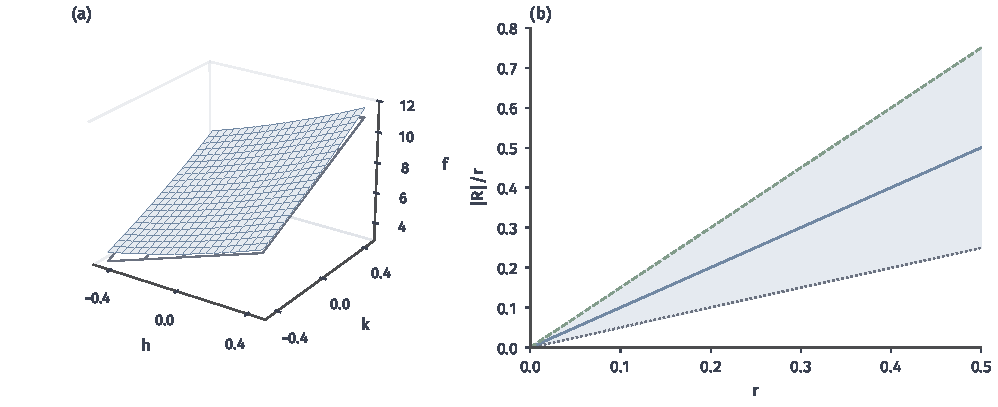
\includegraphics[width=169.0mm]{figures/00-shared/mathematical-preliminaries-upper/00-shared/matplotlib/chapter3-concept-processes/total-differential-remainder.pdf}
 \caption{(a) 二次函数在$(1,2)$附近，灰网格是切平面$P=7+4h+5k$，蓝面是$f(1+h,2+k)$。(b) 令$r=\sqrt{h^2+k^2}$，余项$R=h^2+hk+k^2$满足$r/2\leq R/r\leq3r/2$；阴影给出所有方向的完整范围，三条线是其中的代表值。共同上界随$r\to0$趋零，才保证任意方向都适用同一个线性近似。}
 \label{fig:analysis-process-total-differential-remainder}
\end{figure*}

\paragraph{偏导数连续给出的充分条件}
按定义验证可微，需要估计余项，通常不方便。另一种判别只检查偏导数：如果各坐标的变化率在基点附近连续变化，就可以沿坐标逐段走，用它们共同控制全部坐标增量。
与定理~\ref{thm:multivariable-differentiable-necessary}的必要条件不同，这项条件直接保证全微分存在。
\begin{theorem}[偏导数连续与可微性]
\label{thm:multivariable-continuous-partials-sufficient}
设$f:U\to\mathbb R$，$U$开，$\bm a\in U$。若各一阶偏导数在$\bm a$的某个邻域内存在，并在$\bm a$处连续，则$f$在$\bm a$处可微。
\end{theorem}
\begin{proof}
先看$d=2$。从$(a_1,a_2)$走到$(a_1+h_1,a_2+h_2)$，可以先竖直走、再水平走：
\[
 \begin{aligned}
 &f(a_1+h_1,a_2+h_2)-f(a_1,a_2)\\
 &=\bigl[f(a_1+h_1,a_2+h_2)-f(a_1,a_2+h_2)\bigr]\\
 &\quad+\bigl[f(a_1,a_2+h_2)-f(a_1,a_2)\bigr].
 \end{aligned}
\]
第一个方括号只改变第一个坐标，对一元函数$s\mapsto f(s,a_2+h_2)$用中值定理，得到它等于$\partial_1f(\bm\xi_1)h_1$，其中$\bm\xi_1$在这段水平线段上；第二个方括号同理等于$\partial_2f(\bm\xi_2)h_2$，$\bm\xi_2$在竖直线段上。这里用到$\bm h$足够小时两段都在偏导数存在的邻域内。

一般的$d$同样把$\bm a$到$\bm a+\bm h$的增量拆成$d$段，每段只改一个坐标，一元中值定理将第$j$段增量写成$\partial_jf(\bm\xi_j)h_j$，$\bm\xi_j$是第$j$段上的中间点。
减去候选线性项后，误差为$\sum_j\bigl(\partial_jf(\bm\xi_j)-\partial_jf(\bm a)\bigr)h_j$，因此
\[
 \begin{aligned}
 &\left|f(\bm a+\bm h)-f(\bm a)-\sum_{j=1}^d\partial_j f(\bm a)h_j\right|\\
 &\qquad\leq \max_j\left|\partial_j f(\bm\xi_j)-\partial_j f(\bm a)\right|
       \sum_{j=1}^d|h_j|
 =o(\lVert\bm h\rVert_2).
 \end{aligned}
\]
最后一步有两个依据：当$\bm h\to\bm0$时，所有中间点到$\bm a$的距离都不超过$\lVert\bm h\rVert_2$，偏导数在$\bm a$处连续，使最大值一项趋于零；另一方面$\sum_j|h_j|\leq\sqrt d\lVert\bm h\rVert_2$。
这样，各坐标方向上的变化就拼成了同一个有效的全微分。
\end{proof}
偏导数连续只是充分条件：可微仅要求函数增量具有统一的一阶近似，不要求这些系数随基点连续变化。实际计算中，若各偏导数在所论开集上由连续的表达式给出，例如多项式、分母非零的有理函数，以及它们与指数、正弦等连续函数的复合，就可以直接断定可微。

\paragraph{连续可微函数}
若还希望各点的一阶系数，即梯度，随基点连续变化，就需在一个范围内同时控制偏导数。
实值函数的各一阶偏导数在开集$U$上存在且连续时，称它在$U$上连续可微，记为$C^1(U)$；$C^k(U)$表示直至$k$阶的各偏导数都存在且连续。
定理~\ref{thm:multivariable-continuous-partials-sufficient}保证$C^1$函数处处可微，逆向并不成立，一元函数已经足以说明这一点。
\begin{example}[处处可微而导数无界]
\label{ex:multivariable-differentiable-not-c1}
在实轴上令$r(0)=0$，$x\neq0$时令$r(x)=x^2\sin(1/x^2)$。
由于$|r(h)/h|=|h\sin(1/h^2)|\leq|h|\to0$，有$r'(0)=0$；非零点按运算法则求导，得到
\[
 r'(x)=2x\sin(1/x^2)-\frac{2}{x}\cos(1/x^2).
\]
取$x_n=(2\pi n)^{-1/2}$，则$1/x_n^2=2\pi n$，$\sin$项为$0$、$\cos$项为$1$，于是$r'(x_n)=-2/x_n\to-\infty$。所以$r$处处可微，$r'$却在$0$附近无界，在$0$处不连续。
直观上，$r$的振幅被$x^2$压到零，图像在原点与横轴相切；但振荡越来越快，切线斜率剧烈摆动。
在多元情形令$f(\bm x)=r(x_1)$，就得到处处可微而非连续可微的标量函数。
\end{example}

这个例子还说明可微不保证局部Lipschitz连续：若$r$在原点的某个邻域内以$L$为Lipschitz常数，该邻域内每个差商的绝对值都不超过$L$，各点导数也就满足$|r'|\leq L$，与$r'(x_n)\to-\infty$矛盾。

\paragraph{条件之间的蕴含关系}
由必要条件与充分判别，可以把这些要求放在一起比较：
\[
 \begin{gathered}
 f\text{在}\bm a\text{的某邻域内连续可微}
 \ \Longrightarrow\ f\text{在}\bm a\text{处可微},\\
 f\text{在}\bm a\text{处可微}
 \ \Longrightarrow\ \text{全部双侧方向导数存在}
 \ \Longrightarrow\ \text{全部偏导数存在}.
 \end{gathered}
\]
第一条由定理~\ref{thm:multivariable-continuous-partials-sufficient}得到，第二条由定理~\ref{thm:multivariable-differentiable-necessary}得到，最后一条只须在全部方向中取坐标方向$\bm e_j$。
同一定理还说明，可微蕴含连续，并使方向导数关于方向成为同一个线性映射$\bm v\mapsto\nabla f(\bm a)^\top\bm v$。
第一行的前提涉及$\bm a$的整个邻域，其余条件只涉及基点$\bm a$本身；示例~\ref{ex:multivariable-differentiable-not-c1}已经说明，即使处处可微，也不能反推连续可微。

一元函数在一点的导数存在就等价于可微，因为实轴上只有一条直线可走。多元函数还须协调无穷多个输入方向以及弯曲的趋近路径，所以第二行的两个逆命题也不成立，以下依次给出反例。

\paragraph{偏导数存在不保证可微}
先看坐标偏导数：它们只约束两条坐标切片，并未控制其余方向或路径。
\begin{example}[偏导数存在但不可微]
\label{ex:analysis-partials-not-differentiable}
定义$f:\mathbb{R}^2\to\mathbb{R}$为
\[
 f(x,y)=
 \begin{cases}
  \dfrac{xy}{\sqrt{x^2+y^2}}, & (x,y)\neq(0,0),\\[6pt]
  0, & (x,y)=(0,0).
 \end{cases}
\]
沿两条坐标轴，函数恒为$0$，所以$\partial f/\partial x(0,0)=\partial f/\partial y(0,0)=0$。若$f$在原点可微，由定理~\ref{thm:multivariable-differentiable-necessary}，候选线性部分只能是零映射。可是沿$\bm{h}=(t,t)$，
\[
 \frac{|f(t,t)-f(0,0)|}{\lVert(t,t)\rVert_2}
 =\frac{|t|/\sqrt{2}}{\sqrt{2}|t|}
 =\frac12,
\]
余项与$\lVert\bm{h}\rVert_2$之比不趋于零，故$f$在原点不可微。

用极坐标可以看清曲面的形状：$f=r\cos\theta\sin\theta=\tfrac r2\sin2\theta$。沿每条从原点出发的射线，函数随$r$线性增长，斜率$\tfrac12\sin2\theta$随方向变化。曲面由这些射线组成，像一个起伏的锥面；把它放大任意倍数后形状不变，永远不会变得像一张平面。

沿每个方向$\bm v=(a,b)$，只令$t\downarrow0$的正向方向导数都存在，等于$ab/\sqrt{a^2+b^2}$（零方向取$0$），但它不是关于$\bm v$的线性函数。$t<0$时差商变号，因此$ab\neq0$时双侧方向导数不存在。
最后，由$|xy|/\sqrt{x^2+y^2}\leq\sqrt{x^2+y^2}/2$，$f$在原点连续。
\end{example}

偏导数只看坐标轴，遗漏了其他接近方向；可微则要求曲面放大后接近平面，本例的锥面做不到。这个例子还说明，偏导数存在、全部正向方向导数存在，再加上连续性，都不足以推出可微。方向极限采用单侧还是双侧，必须与所用定义一致；本节定义采用双侧极限。

\paragraph{全部方向导数存在不保证可微}
从坐标切片扩展到所有固定直线，仍需检查两件事：这些变化率能否组成一个线性映射，以及是否具有统一余项。先看缺少线性性的情形。
\begin{example}[方向导数不构成线性映射]
\label{ex:multivariable-nonlinear-directional-derivatives}
在非原点处令$p(x,y)=x^3/(x^2+y^2)$，并令$p(0,0)=0$。
沿$\bm v=(a,b)\neq\bm0$，差商为$p(ta,tb)/t=a^3/(a^2+b^2)$，不依赖$t$，所以双侧方向导数存在且$D_{\bm v}p(0,0)=a^3/(a^2+b^2)$。
取坐标方向得到候选梯度$(1,0)^\top$。若$p$可微，沿$(1,1)^\top$的方向导数应为$(1,0)(1,1)^\top=1$，实际却是$1/(1+1)=1/2$。这些方向变化率无法拼成一个线性映射，所以$p$在原点不可微。
\end{example}

与示例~\ref{ex:analysis-partials-not-differentiable}只有单侧方向极限不同，这里的双侧方向导数全部存在，失败只来自线性性。
即使方向导数全部存在并组成一个线性映射，仍需检查统一余项。
\begin{example}[方向导数全为零仍不可微]
\label{ex:multivariable-linear-directionals-not-differentiable}
在非原点处令$q(x,y)=x^3y/(x^4+y^2)$，并令$q(0,0)=0$。
由$2|x^2y|\leq x^4+y^2$，有$|q(x,y)|\leq|x|/2$，故$q$在原点连续。
对固定方向$(a,b)^\top$，若$b\neq0$，
\[
 \frac{q(ta,tb)}t=\frac{t a^3b}{t^2a^4+b^2}\longrightarrow0;
\]
若$b=0$，差商恒为零。因此所有双侧方向导数都为零，它们组成零线性映射。
可是沿$\bm h=(t,t^2)^\top$，$q(t,t^2)=t^5/(2t^4)=t/2$，从而
\[
 \frac{|q(t,t^2)|}{\lVert(t,t^2)\rVert_2}
 =\frac1{2\sqrt{1+t^2}}\longrightarrow\frac12.
\]
候选零映射不满足全微分的余项条件，$q$在原点不可微。
\end{example}

这与示例~\ref{ex:multivariable-parabola-path-limit}中$g$的情形相同：函数沿抛物线有一道坡，每条直线进入原点时都避开了它。方向导数先固定方向再取极限，全微分则要求对方向随扰动改变的序列也有同一个误差控制。

\paragraph{连续不保证偏导数存在}
反过来，连续性也推不出微分条件。
例如$f(x,y)=|x|$在整个平面上Lipschitz连续，图像沿$y$轴有一道折痕，原点关于$x$的双侧偏导数不存在，因此在那里不可微。
偏导数存在同样推不出连续：示例~\ref{ex:multivariable-path-limits}中原点置零的$xy/(x^2+y^2)$沿坐标轴恒为零，两个偏导数存在，但它在原点不连续。
因此连续与偏导数存在之间互不蕴含；可微则同时保证二者。

\paragraph{梯度与线性近似的使用条件}
上述反例区分了梯度的两种用途。仅有偏导数时，梯度只是坐标变化率排成的向量；确认可微以后，才可用它统一预测增量，用内积计算任意方向导数，并把它解释为最快上升的方向。
连续偏导数提供方便的充分判别，却不是必要条件；不满足该判别时，应回到全微分的统一余项定义检查。
讨论向量值函数时，同样对各个标量输出分量分别检查，再组成Jacobian矩阵及复合微分。

\subsection{微分的运算法则}

本小节的$f,g$都在同一开集内定义，并在基点$\bm a$处可微，$c$为固定实数。
各法则的证明方法相同：把各自的一阶展开代入，整理出关于$\bm h$的线性项，再确认剩下的部分仍是$o(\lVert\bm h\rVert_2)$。这样既得到新函数可微，也读出了它的全微分。

\paragraph{和的微分}
把两个一阶展开相加，
\[
 (f+g)(\bm a+\bm h)=(f+g)(\bm a)+\bigl(\mathrm df_{\bm a}+\mathrm dg_{\bm a}\bigr)(\bm h)+o(\lVert\bm h\rVert_2),
\]
两个线性映射之和仍是线性映射，两个$o(\lVert\bm h\rVert_2)$余项之和仍是$o(\lVert\bm h\rVert_2)$，因此
\[
 \begin{gathered}
\mathrm d(f+g)=\mathrm df+\mathrm dg\\
\nabla(f+g)=\nabla f+\nabla g.
 \end{gathered}
\]

\paragraph{差的微分}
把加号换成减号，同样的论证给出
\[
 \begin{gathered}
\mathrm d(f-g)=\mathrm df-\mathrm dg\\
\nabla(f-g)=\nabla f-\nabla g.
 \end{gathered}
\]

\paragraph{数乘的微分}
固定系数$c$只会缩放线性项与余项，故
\[
 \begin{gathered}
\mathrm d(cf)=c\,\mathrm df\\
\nabla(cf)=c\nabla f,
 \end{gathered}
\]
包括$c=0$的常函数情形。

\paragraph{积的微分}
记$R_f,R_g$为两个一阶展开的余项，都是$o(\lVert\bm h\rVert_2)$。相乘得
\[
 \begin{aligned}
 f(\bm a+\bm h)g(\bm a+\bm h)
 &=\bigl(f(\bm a)+\mathrm df(\bm h)+R_f\bigr)\bigl(g(\bm a)+\mathrm dg(\bm h)+R_g\bigr)\\
 &=f(\bm a)g(\bm a)+g(\bm a)\,\mathrm df(\bm h)+f(\bm a)\,\mathrm dg(\bm h)+(\text{其余各项}).
 \end{aligned}
\]
其余各项要么含有余项$R_f,R_g$乘以有界量，要么是两个线性增量的乘积$\mathrm df(\bm h)\,\mathrm dg(\bm h)=O(\lVert\bm h\rVert_2^2)$，都是$o(\lVert\bm h\rVert_2)$。因此乘积可微，且
\[
 \mathrm d(fg)=g(\bm a)\,\mathrm df+f(\bm a)\,\mathrm dg.
\]
这与一元的$(fg)'=f'g+fg'$形式相同：两个因子各自变化，一阶上贡献可以相加，两个变化同时发生的部分是高阶小量。

\paragraph{商的微分}
设$g(\bm a)\neq0$。可微蕴含连续，所以$g$在$\bm a$附近远离零，$1/g$在$\bm a$附近有定义。记$\delta=g(\bm a+\bm h)-g(\bm a)=\mathrm dg(\bm h)+o(\lVert\bm h\rVert_2)$，它是$O(\lVert\bm h\rVert_2)$。一元函数$1/y$在$g(\bm a)$处的展开给出
\[
 \frac1{g(\bm a)+\delta}=\frac1{g(\bm a)}-\frac{\delta}{g(\bm a)^2}+O(\delta^2).
\]
代入$\delta$的展开，并注意$O(\delta^2)=O(\lVert\bm h\rVert_2^2)$，得到$\mathrm d(1/g)=-\mathrm dg/g(\bm a)^2$。再把$f/g$看成$f\cdot(1/g)$，用积的微分得到
\[
 \mathrm d(f/g)=\frac{g(\bm a)\,\mathrm df-f(\bm a)\,\mathrm dg}{g(\bm a)^2}.
\]
这里分母非零既是定义商函数的条件，也是估计余项的条件。

\paragraph{标量复合函数的微分}
若一元函数$\psi$在$f(\bm a)$处可微，且复合在$\bm a$的邻域内有定义，则$\psi\circ f$在$\bm a$处可微，并且
\[
 \begin{gathered}
\mathrm d(\psi\circ f)=\psi'(f(\bm a))\,\mathrm df\\
\nabla(\psi\circ f)(\bm a)=\psi'(f(\bm a))\nabla f(\bm a).
 \end{gathered}
\]
推导时把内层增量$\delta=f(\bm a+\bm h)-f(\bm a)$代入外层的一元展开$\psi(f(\bm a)+\delta)=\psi(f(\bm a))+\psi'(f(\bm a))\delta+o(|\delta|)$，再把$\delta=\mathrm df(\bm h)+o(\lVert\bm h\rVert_2)$代入。
因为$\delta=O(\lVert\bm h\rVert_2)$，外层余项$o(|\delta|)$仍是$o(\lVert\bm h\rVert_2)$。
例如$\nabla e^{-(x^2+y^2)}=e^{-(x^2+y^2)}(-2x,-2y)^\top$：外层只把内层梯度乘上一个正数，所以复合函数的梯度与$-(x^2+y^2)$的梯度同向，都指向原点。

\paragraph{二次型的微分}
向量自变量的二次型仍是标量函数，机器学习中的平方误差、能量函数等都含有这种结构。考虑$q(\bm{x})=\bm{x}^{\top}\bm{A}\bm{x}=\sum_{i,j}A_{i,j}x_ix_j$，其中$\bm{A}\in\mathbb{R}^{d\times d}$固定。它是有限个乘积的和，乘积法则可以直接使用：把两个$\bm x$看成两个因子，每次只让一个变化，
\begin{align*}
  \mathrm{d}q
  &=
  (\mathrm{d}\bm{x})^{\top}\bm{A}\bm{x}
  +\bm{x}^{\top}\bm{A}\,\mathrm{d}\bm{x}\\
  &=
  \bm{x}^{\top}(\bm{A}^{\top}+\bm{A})\,\mathrm{d}\bm{x}.
\end{align*}
第二步用到$(\mathrm d\bm x)^\top\bm A\bm x$是一个实数，等于自己的转置$\bm x^\top\bm A^\top\mathrm d\bm x$。把$\mathrm dq$写成$\nabla q^\top\mathrm d\bm x$的形式，就读出
\begin{equation}
  \nabla_{\bm{x}}
  \bigl(\bm{x}^{\top}\bm{A}\bm{x}\bigr)
  =
  (\bm{A}+\bm{A}^{\top})\bm{x}.
\label{eq:analysis-quadratic-form-gradient}
\end{equation}
当$\bm{A}$对称时，式~\eqref{eq:analysis-quadratic-form-gradient}化为$2\bm{A}\bm{x}$，与一元的$(ax^2)'=2ax$对应；$\bm A$不对称时直接写成$2\bm{A}\bm{x}$，等于悄悄加入了对称性条件。
例如$\bm A=\begin{bmatrix}0&1\\0&0\end{bmatrix}$时$q=x_1x_2$，直接求偏导得$\nabla q=(x_2,x_1)^\top$，与$(\bm A+\bm A^\top)\bm x$一致；而$2\bm A\bm x=(2x_2,0)^\top$是错的。

\subsection{梯度的几何意义}

全微分是扰动上的线性泛函。指定内积以后，它有唯一的内积表示向量，这就是梯度；在非标准坐标中，要用Gram矩阵把坐标偏导换成该向量的坐标。

方向导数公式还说明了梯度指向哪里。

设$f$在$\bm a$处可微，对单位方向$\bm u$，由内积不等式，$D_{\bm u}f(\bm a)=\nabla f(\bm a)^\top\bm u\leq\lVert\nabla f(\bm a)\rVert_2$。
梯度非零时，取$\bm u=\nabla f(\bm a)/\lVert\nabla f(\bm a)\rVert_2$即达到等号，所以梯度方向是局部上升最快的单位方向。
这些结论都需要可微性，不能只由梯度向量存在推出。

图~\ref{fig:analysis-process-gradient-level-curves}用同一个二次函数比较梯度方向、等值曲线切向及另一个单位方向。
\begin{figure}[!htbp]
 \centering
 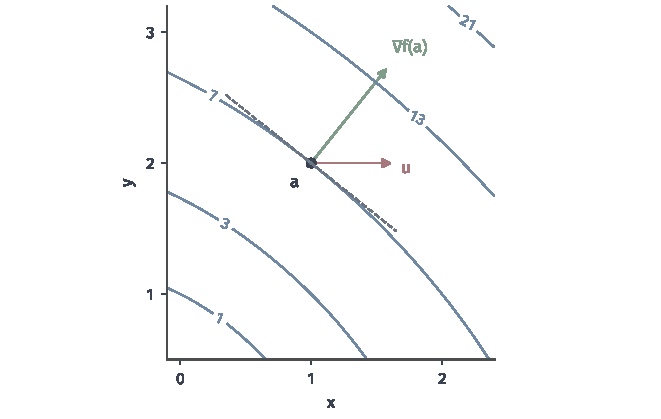
\includegraphics[width=112.0mm]{figures/00-shared/mathematical-preliminaries-upper/00-shared/matplotlib/chapter3-concept-processes/gradient-level-curves.pdf}
 \caption{$f=x^2+xy+y^2$的等值曲线，标注为函数值；基点$a=(1,2)$处$\nabla f=(4,5)^\top$，图中绿箭头按$0.15$倍绘制。灰虚线沿$(5,-4)^\top$，与梯度垂直，因而与经过$a$的等值曲线相切；红箭头为$u=(1,0)^\top$。比较最快上升方向时须先归一化，不能直接比较图中箭头长度。}
 \label{fig:analysis-process-gradient-level-curves}
\end{figure}

\subsection{中值估计与局部Lipschitz性}

导数控制一点处的变化；要估计两点之间的有限变化，可以沿连接两点的线段把函数限制为一元函数，再使用一元中值定理。前提是整条线段都在定义域内。
记$[\bm x,\bm y]=\{\bm x+t(\bm y-\bm x):0\leq t\leq1\}$为连接两点的线段。
\begin{theorem}[多元标量函数的中值公式]
\label{thm:multivariable-scalar-mean-value}
设$f$在包含$[\bm x,\bm y]$的开集上可微，$\bm x\neq\bm y$。则存在$\theta\in(0,1)$使
\[
 f(\bm y)-f(\bm x)=\nabla f(\bm x+\theta(\bm y-\bm x))^\top(\bm y-\bm x).
\]
\end{theorem}
\begin{proof}
令$\phi(t)=f(\bm x+t(\bm y-\bm x))$，$t\in[0,1]$，它是$f$在线段上的一元切片。$\phi'(t)$就是$f$在点$\bm x+t(\bm y-\bm x)$处沿$\bm y-\bm x$的方向导数，由定理~\ref{thm:multivariable-differentiable-necessary}，$\phi'(t)=\nabla f(\bm x+t(\bm y-\bm x))^\top(\bm y-\bm x)$。
对$\phi$在$[0,1]$上使用一元中值定理，$\phi(1)-\phi(0)=\phi'(\theta)$，这就是所述等式。
\end{proof}
等式说明，两点之间的平均变化率等于线段上某一点沿该方向的瞬时变化率，这是一元“平均斜率等于某点切线斜率”的直接推广。
例如$f(x,y)=x^2+y^2$，$\bm x=(0,0)$、$\bm y=(1,1)$，左侧为$2$；右侧为$\nabla f(\theta,\theta)^\top(1,1)^\top=4\theta$，取$\theta=1/2$即相等，中值点恰为线段中点。

\paragraph{局部Lipschitz性}

中值公式把有限增量写成某点梯度与位移的内积。若梯度的长度有统一上界，就能用输入距离的常数倍控制输出变化，这就是多元情形的Lipschitz条件。优化中常用它由步长控制函数值的变化。
\begin{definition}[多元函数的Lipschitz条件]
\label{def:multivariable-lipschitz}
设$D\subseteq\mathbb R^d$，$f:D\to\mathbb R$。若存在有限常数$L\geq0$，使
\[
 |f(\bm x)-f(\bm y)|\leq L\lVert\bm x-\bm y\rVert_2\qquad(\bm x,\bm y\in D),
\]
称$f$在$D$上Lipschitz连续，$L$称为Lipschitz常数。若每点都有一个邻域使$f$在其中Lipschitz连续（常数可随邻域改变），称$f$局部Lipschitz连续。
\end{definition}
这与一元定义只差把$|x-y|$换成欧氏距离。

例如线性函数$f(\bm x)=\bm a^\top\bm x$满足$|f(\bm x)-f(\bm y)|=|\bm a^\top(\bm x-\bm y)|\leq\lVert\bm a\rVert_2\lVert\bm x-\bm y\rVert_2$，Lipschitz常数可取$\lVert\bm a\rVert_2$。

欧氏范数$f(\bm x)=\lVert\bm x\rVert_2$由三角不等式满足$|\lVert\bm x\rVert_2-\lVert\bm y\rVert_2|\leq\lVert\bm x-\bm y\rVert_2$，常数为$1$，尽管它在原点不可微。

梯度界要转化为Lipschitz常数，还需要两点之间的线段留在定义域内。集合$D$称为凸集，是指其中任意两点之间的线段都含于$D$。在凸开集上，梯度长度的统一上界恰好就是Lipschitz常数。
\begin{theorem}[梯度有界与Lipschitz条件]
\label{thm:multivariable-gradient-lipschitz}
设$U\subseteq\mathbb R^d$为凸开集，$f:U\to\mathbb R$可微。则$f$在$U$上以$L$为Lipschitz常数，当且仅当$\lVert\nabla f(\bm x)\rVert_2\leq L$对所有$\bm x\in U$成立。
\end{theorem}
\begin{proof}
若梯度长度不超过$L$，任取$\bm x\neq\bm y$，凸性保证线段$[\bm x,\bm y]\subseteq U$。由中值公式与内积不等式，
\[
 |f(\bm y)-f(\bm x)|=\bigl|\nabla f(\bm\xi)^\top(\bm y-\bm x)\bigr|\leq\lVert\nabla f(\bm\xi)\rVert_2\lVert\bm y-\bm x\rVert_2\leq L\lVert\bm y-\bm x\rVert_2.
\]
反过来，设$f$以$L$为Lipschitz常数。固定$\bm x$，若$\nabla f(\bm x)\neq\bm0$，取单位方向$\bm u=\nabla f(\bm x)/\lVert\nabla f(\bm x)\rVert_2$，则
\[
 \lVert\nabla f(\bm x)\rVert_2=D_{\bm u}f(\bm x)=\lim_{t\downarrow0}\frac{f(\bm x+t\bm u)-f(\bm x)}t\leq\lim_{t\downarrow0}\frac{Lt}t=L.
\]
梯度为零时不等式自然成立。
\end{proof}
几何上，若坡度处处不超过$L$，沿直线走过距离$\rho$，高度最多改变$L\rho$；反过来，Lipschitz常数也限制了每一点最陡方向的坡度。
例如$f(x,y)=\sin x+\cos y$满足$\lVert\nabla f\rVert_2=\sqrt{\cos^2x+\sin^2y}\leq\sqrt2$，所以它在整个平面上以$\sqrt2$为Lipschitz常数。

定理中的凸性不能省略。在不凸的区域上，梯度可以处处很小，函数值却在两个很近的点之间相差很大。
\begin{example}[非凸区域上梯度有界而不Lipschitz]
\label{ex:multivariable-nonconvex-lipschitz-failure}
取去掉负$x$轴的环形区域$D=\{1<\lVert\bm x\rVert_2<2\}\setminus\{(x,0):x<0\}$，令$f(\bm x)$为点$\bm x$的极角，取值于$(-\pi,\pi)$。$f$在$D$上可微，$\lVert\nabla f\rVert_2=1/r<1$，坡度处处小于$1$。
但取负$x$轴两侧的点$(-1.5,\pm\varepsilon)$，两点距离为$2\varepsilon$，极角却分别接近$\pi$与$-\pi$，相差接近$2\pi$。令$\varepsilon\to0$，函数值之差与距离之比无界，所以$f$在$D$上不是Lipschitz函数。
\end{example}

连接这两点的直线段穿过被去掉的负$x$轴，不在$D$内，中值公式无法使用；$D$内连接两点的路径必须绕过原点，长度远大于$2\varepsilon$。梯度界只能沿含于定义域的线段转化为函数值之差的界。

局部情形同理。若$f\in C^1(U)$，在每个基点附近取一个包含在$U$内的闭球。连续函数$\lVert\nabla f\rVert_2$在这个闭有界集上有界（定理~\ref{thm:multivariable-extreme-value}），因而在同心的开球上也有界；开球是凸开集，故由定理~\ref{thm:multivariable-gradient-lipschitz}，$f$在这个开球上Lipschitz连续，从而局部Lipschitz连续。
局部常数不自动给出全域共同常数：$f(x,y)=x^2$连续可微，但$\lVert\nabla f\rVert_2=2|x|$在全平面无界，因而它不是全域Lipschitz函数。

\section{多元标量函数的高阶微分}
\label{sec:multivariable-curvature-error}

一阶微分用切平面描述局部变化，却看不出曲面向哪边弯：碗底、山顶和马鞍点处的切平面都是水平的。高阶微分记录一阶系数本身怎样变化，从而描述弯曲。
本节先把二阶偏导数集中为Hessian矩阵，再用Taylor公式建立二阶近似，最后据此判断驻点的局部极值类型。

\subsection{二阶偏导数、Hessian与高阶微分}

一阶偏导数本身仍是多元标量函数，可以再次求偏导。这里记$f_{x_i x_j}=\partial_j(\partial_i f)$，即先对$x_i$、再对$x_j$求导。
$f_{xx}$描述$x$方向切片的斜率沿$x$方向怎样变化，即该切片的弯曲；混合偏导数$f_{xy}$描述$x$方向的斜率在沿$y$方向移动时怎样变化，即曲面的扭转。

对$f(x,y)=x^2+xy+y^2$，有$f_{xx}=2$、$f_{xy}=f_{yx}=1$、$f_{yy}=2$。又如$f(x,y)=xy$，$x$方向切片的斜率是$y$，向北每走一单位，这个斜率就增加$1$，故$f_{xy}=1$，而$f_{xx}=f_{yy}=0$：每条坐标切片都是直线，曲面却是扭曲的。
这两个例子中$f_{xy}=f_{yx}$，但一般函数的混合偏导数能否交换次序，需要额外条件。

\paragraph{混合偏导数的交换}
分别沿两个坐标求导时，先后次序未必无关。
\begin{example}[混合偏导数与求导次序有关]
\label{ex:multivariable-mixed-partials-differ}
令$f(0,0)=0$，非原点处令
\[
 f(x,y)=\frac{xy(x^2-y^2)}{x^2+y^2}.
\]
对$y\neq0$，因为$f(0,y)=0$，
\[
 f_x(0,y)=\lim_{h\to0}\frac{f(h,y)}h=\lim_{h\to0}\frac{y(h^2-y^2)}{h^2+y^2}=-y;
\]
又$f$在$x$轴上恒为$0$，故$f_x(0,0)=0$，公式$f_x(0,y)=-y$在$y=0$时也成立。同样算得$f_y(x,0)=x$对所有$x$成立。于是
\[
 \begin{gathered}
f_{xy}(0,0)=\frac{\mathrm d}{\mathrm dy}(-y)\Big|_{y=0}=-1\\
f_{yx}(0,0)=\frac{\mathrm d}{\mathrm dx}x\Big|_{x=0}=1,
 \end{gathered}
\]
两个次序给出不同结果。
\end{example}

定理~\ref{thm:multivariable-mixed-partials}将说明，混合偏导数在基点连续时两种次序一定相同；因此本例的混合偏导数不可能都在原点连续。
\begin{theorem}[混合偏导数的交换]
\label{thm:multivariable-mixed-partials}
设$f$在$\bm a$的某个开邻域内有一阶偏导数$\partial_i f,\partial_j f$，混合偏导数$\partial_j\partial_i f,\partial_i\partial_j f$在该邻域存在并在$\bm a$处连续，则
\[
 \partial_j\partial_i f(\bm a)=\partial_i\partial_j f(\bm a).
\]
特别地，$C^2$函数的混合偏导数处处可以交换。
\end{theorem}
\begin{proof}
固定其他坐标，只需讨论二元函数在$(a,b)$处的情形。对小的非零$h,k$考察小矩形四个顶点上的二阶差分
\[
 \Delta(h,k)=f(a+h,b+k)-f(a+h,b)-f(a,b+k)+f(a,b).
\]
它可以按两种方式分组：先比较上下两边的差，或先比较左右两边的差，两种分组各给出一个混合偏导数。

令$\phi(x)=f(x,b+k)-f(x,b)$，则$\Delta=\phi(a+h)-\phi(a)$。先对$\phi$用一元中值定理，得到$\Delta=h\phi'(\xi)=h[f_x(\xi,b+k)-f_x(\xi,b)]$；再对$y\mapsto f_x(\xi,y)$使用一次中值定理，得到
\[
 \Delta=h[f_x(\xi,b+k)-f_x(\xi,b)]=hk f_{xy}(\xi,\eta),
\]
其中$\xi$在$a,a+h$之间、$\eta$在$b,b+k$之间。改用$\psi(y)=f(a+h,y)-f(a,y)$先沿$y$方向拆分，同样得到$\Delta=hk f_{yx}(\xi',\eta')$。
于是$f_{xy}(\xi,\eta)=f_{yx}(\xi',\eta')$。令$h,k\to0$，两个中间点都趋于$(a,b)$，连续性使两种混合偏导数在该点相等。
\end{proof}
示例~\ref{ex:multivariable-mixed-partials-differ}说明，只有混合偏导数存在而没有这些连续性条件时，结论可能失败。

\paragraph{Hessian矩阵}
把全部二阶偏导数排成一个方阵，就得到记录二阶信息的矩阵，它的行、列分别对应先后两次求导的输入坐标。
\begin{definition}[Hessian矩阵]
\label{def:multivariable-hessian}
若$f:U\to\mathbb R$在$\bm x$附近有一阶偏导数，且各$\partial_j\partial_i f(\bm x)$存在，则称
\[
 \nabla^2f(\bm x)=\bigl[\partial_j\partial_i f(\bm x)\bigr]_{i,j=1}^d
\]
为$f$在该点的\term{Hessian矩阵}（Hessian matrix）。
\end{definition}
第$i$行是第$i$个偏导数$\partial_if$的梯度（转置后），所以Hessian也可以理解为“梯度的梯度”：它说明当基点移动时，梯度向量怎样变化。
二阶偏导数存在本身尚不保证梯度映射$\nabla f$具有统一的线性近似；二阶可微要求$\nabla f$本身可微。
$C^2$是保证二阶可微的充分条件，且由定理~\ref{thm:multivariable-mixed-partials}，此时Hessian对称。对$x^2+xy+y^2$，Hessian就是$\begin{bmatrix}2&1\\1&2\end{bmatrix}$。

一元函数的二阶导数描述曲线向上还是向下弯；多元函数可以沿每个方向分别看。若$f\in C^2$，沿直线$t\mapsto f(\bm x+t\bm v)$求两次导数，在$t=0$处得到
\[
 \bm v^\top\nabla^2f(\bm x)\bm v
 =\sum_{i=1}^d\sum_{j=1}^d \partial_j\partial_i f(\bm x)v_i v_j.
\]
这一计算的依据在定理~\ref{thm:multivariable-second-order-taylor}的证明中给出。这个实数二次型衡量一阶斜率沿给定方向的变化，即沿方向$\bm v$截出的切片曲线的弯曲：为正时向上弯，为负时向下弯。

二次函数的Hessian可以直接读出。对
\[
 f(\bm{x})=\frac12\bm{x}^{\top}\bm{A}\bm{x}+\bm{b}^{\top}\bm{x}+c,
\]
只有$\bm{A}$的对称部分影响函数值，因为$\bm x^\top\bm A\bm x$与其转置$\bm x^\top\bm A^\top\bm x$相等。令$\bm{H}=(\bm{A}+\bm{A}^{\top})/2$，由式~\eqref{eq:analysis-quadratic-form-gradient}，$\nabla f(\bm{x})=\bm{H}\bm{x}+\bm{b}$，再求一次导得$\nabla^2f(\bm{x})=\bm{H}$。二次函数的Hessian是常数矩阵，各处弯曲相同。

例如$\bm H=\operatorname{diag}(2,100)$时，方向二次型为$2v_1^2+100v_2^2$：沿两个坐标方向都向上弯，但第二个方向的二阶变化率是第一个的$50$倍。函数图像是一个狭长的山谷：等值曲线是椭圆，沿$x_1$方向的半轴是沿$x_2$方向的$\sqrt{50}\approx7.1$倍。优化中这种形状会让梯度方法在陡峭方向来回摆动。
若改为$\operatorname{diag}(2,-100)$，两个坐标方向的弯曲方向便相反，图像是马鞍形。

这些情形按二次型的符号分类。第~\ref{sec:prelim-common-matrices}节已定义正定与半正定矩阵，这里把这些概念用于Hessian，并补充不定的情形：对实对称矩阵$\bm H$，若每个非零$\bm v$都有$\bm v^\top\bm H\bm v>0$，称$\bm H$正定；
若只要求$\bm v^\top\bm H\bm v\geq0$，则称半正定。
把不等号反向得到负定与半负定；若既存在使二次型为正的方向，又存在使它为负的方向，则称矩阵不定。
这些名称说明全部方向或某些方向上的曲率符号：正定对应各方向都向上弯的碗形，负定对应倒扣的碗，不定对应马鞍。

判断定性需要检查整个二次型，不能只看对角元素。
\begin{example}[用二次型判断Hessian的定性]
\label{ex:multivariable-hessian-definiteness}
对$\bm H=\begin{bmatrix}2&1\\1&2\end{bmatrix}$，配方得
\[
 \bm v^\top\bm H\bm v=2v_1^2+2v_1v_2+2v_2^2=(v_1+v_2)^2+v_1^2+v_2^2,
\]
非零$\bm v$时为正，所以$\bm H$正定。
对$\begin{bmatrix}1&2\\2&1\end{bmatrix}$，两个对角元都为正，但取$\bm v=(1,-1)^\top$得$1-4+1=-2<0$，取$\bm v=(1,1)^\top$得$6>0$，所以矩阵不定。
\end{example}

第二个矩阵的对角元只说明沿坐标轴向上弯；沿对角线$y=-x$，曲面却向下弯。

\paragraph{高阶微分的多线性形式}

Hessian不仅是一张二阶偏导数组，还规定了两个扰动方向之间的配对。

对$C^2$标量函数，记$H_f=\nabla^2f$，定义
\[
 D^2f_{\bm x}[\bm h,\bm k]=\bm h^\top H_f(\bm x)\bm k.
\]
它对两个方向分别线性，且由混合偏导相等而对称。二阶微分作用于两个不同方向，记录一个方向的变化率如何随另一个方向改变；把两个方向都取成$\bm h$，才得到Taylor公式中的二次项。

一般地，$f$为$C^r$时，令
\[
 D^rf_{\bm x}[\bm h_1,\ldots,\bm h_r]
 =\sum_{i_1,\ldots,i_r=1}^d
 \frac{\partial^rf}{\partial x_{i_1}\cdots\partial x_{i_r}}(\bm x)
 (h_1)_{i_1}\cdots(h_r)_{i_r}.
\]
有限和中的每一项对每个方向分别线性，所以这定义一个$r$重线性形式。连续混合偏导的交换使它对方向次序对称；坐标数组只是这个多线性作用在基下的记录。向量值微分建立后，也可以把它理解为对前一级微分再次求导。

例如$f(x,y)=x^2y$在$(1,2)$处的Hessian为$\left[\begin{smallmatrix}4&2\\2&0\end{smallmatrix}\right]$。方向$\bm h=(h_1,h_2)^\top$上的二次变化为$4h_1^2+4h_1h_2$；其中混合项说明两个坐标同时变化时，不能把两条坐标轴上的一元展开简单相加。

\subsection{多元Taylor展开与余项}

一元Taylor公式用导数构造多项式近似。把多个坐标同时改变的位移看成一条线段上的参数变化，就能沿这条线段使用一元Taylor公式。
所得公式针对标量输出：一次项给出切平面，二次项是一个实数二次型，补上曲面的弯曲。沿整条线段使用带Lagrange余项的一元公式，得到中间点形式的余项；再利用二阶偏导数在基点的连续性，得到小量形式的余项。
\begin{theorem}[多元标量函数的二阶Taylor公式]
\label{thm:multivariable-second-order-taylor}
设$f\in C^2(U)$，$U\subseteq\mathbb R^d$开，线段$[\bm x,\bm x+\bm h]\subset U$。若$\bm h\neq\bm 0$，则存在$\theta\in(0,1)$使
\begin{equation}
 f(\bm x+\bm h)=f(\bm x)+\nabla f(\bm x)^\top\bm h
 +\frac12\bm h^\top\nabla^2f(\bm x+\theta\bm h)\bm h.
\label{eq:analysis-second-order-taylor}
\end{equation}
对固定$\bm x\in U$，当$\bm h\to\bm 0$时还有
\begin{equation}
 f(\bm x+\bm h)=f(\bm x)+\nabla f(\bm x)^\top\bm h
 +\frac12\bm h^\top\nabla^2f(\bm x)\bm h+o(\lVert\bm h\rVert_2^2).
\label{eq:analysis-second-order-local-model}
\end{equation}
\end{theorem}
\begin{proof}
令$\phi(t)=f(\bm x+t\bm h)$。由定理~\ref{thm:multivariable-differentiable-necessary}的方向导数公式，$\phi'(t)=\nabla f(\bm x+t\bm h)^\top\bm h=\sum_i\partial_if(\bm x+t\bm h)h_i$。
每个$\partial_if$属于$C^1$，因而可微；对它再用一次方向导数公式，$\frac{\mathrm d}{\mathrm dt}\partial_if(\bm x+t\bm h)=\sum_j\partial_j\partial_if(\bm x+t\bm h)h_j$。相加得$\phi''(t)=\sum_{i,j}\partial_j\partial_if(\bm x+t\bm h)h_ih_j=\bm h^\top\nabla^2f(\bm x+t\bm h)\bm h$。
对$\phi$在$[0,1]$上使用带Lagrange余项的一元Taylor定理，$\phi(1)=\phi(0)+\phi'(0)+\tfrac12\phi''(\theta)$，即得第一式。

第二式要把中间点处的Hessian换成基点处的Hessian，并估计替换误差。$\theta\in(0,1)$可以随$\bm h$变化，但中间点$\bm x+\theta\bm h$到$\bm x$的距离不超过$\lVert\bm h\rVert_2$；Hessian各元素又在$\bm x$处连续，所以$\bm h\to\bm 0$时
$\lVert\nabla^2f(\bm x+\theta\bm h)-\nabla^2f(\bm x)\rVert_F\to0$。
对任意方阵$\bm B$，对$\sum_{i,j}B_{i,j}h_i h_j$使用有限和的Cauchy--Schwarz不等式，得到$|\bm h^\top\bm B\bm h|\leq\lVert\bm B\rVert_F\lVert\bm h\rVert_2^2$。取$\bm B$为两个Hessian之差，替换产生的误差不超过$\tfrac12\lVert\bm B\rVert_F\lVert\bm h\rVert_2^2=o(\lVert\bm h\rVert_2^2)$，得到第二式。
\end{proof}
用一个具体函数可以比较一阶近似与二阶近似的误差。
\begin{example}[指数函数的二阶Taylor近似]
\label{ex:multivariable-exponential-taylor}
令$f(x,y)=e^{x+y}$。在原点，函数值为$1$，梯度为$(1,1)^\top$，Hessian的各元素均为$1$，对应的二次型为$h^2+2hk+k^2=(h+k)^2$。由式~\eqref{eq:analysis-second-order-local-model}，
\[
 e^{h+k}=1+h+k+\frac12(h+k)^2+o(h^2+k^2).
\]
取$h=k=0.1$，实际值$e^{0.2}\approx1.22140$。切平面给出$1.2$，误差约$0.021$；加上二次项给出$1.22$，误差降到约$0.0014$。
\end{example}

一次项描述切平面，二次项补上沿位移方向的弯曲，所以加入二次项后误差明显减小。
式~\eqref{eq:analysis-second-order-local-model}则是局部结论。若要在一个区域内给出统一的余项界，还需在整个区域上控制Hessian的变化，例如假设Hessian满足Lipschitz条件；仅凭一点处的二阶导数不能得到这样的界。

若希望保留整条位移线段上的曲率，可以直接使用一元Taylor积分余项式~\eqref{eq:analysis-taylor-integral-remainder}。
在同一$C^2$条件下，令$\phi(t)=f(\bm x+t\bm h)$，取该式的$r=1$；把定理证明中算出的$\phi'$与$\phi''$代入，得到不挑选中间点的Taylor积分余项：
\[
 f(\bm{x}+\bm{h})
 =f(\bm{x})+\nabla f(\bm{x})^{\top}\bm{h}
 +\int_0^1(1-t)\,\bm{h}^{\top}\nabla^2f(\bm{x}+t\bm{h})\bm{h}\,\mathrm{d}t.
\]
权重$1-t$在起点$t=0$处最大、在终点处为零，所以越靠近位移起点的曲率对有限增量贡献越多。该表达式与式~\eqref{eq:analysis-second-order-taylor}描述同一有限变化，但不挑选中间点，而是保留整条线段上的曲率信息。

\subsection{驻点附近的函数形状}

Taylor公式把函数增量写成梯度项、Hessian二次型与高阶余项之和，因此梯度与Hessian的条件可以转化为原函数的极值结论。
先回顾极值的定义。若存在$\bm x^\star$的一个邻域，使其中定义域内的点的函数值都不小于$f(\bm x^\star)$，就称$\bm x^\star$为局部极小点；若邻域中其他点的函数值均严格更大，则称为严格局部极小点；局部极大点与严格局部极大点用反向不等式定义。
本小节只考察开集内部的点，不涉及约束。

\paragraph{局部极值的一阶必要条件}
一元函数在内部极值点处导数为零（Fermat条件）。把多元函数限制在任意一条过极值点的直线上，该点仍是所得一元函数的极值点，所以每个方向上的导数都必须为零。
几何上，这表示极值点处的切平面是水平的。
\begin{theorem}[局部极值的一阶必要条件]
\label{thm:multivariable-extremum-first-order}
设$f:U\to\mathbb R$在开集$U$内的点$\bm x^\star$处可微，且该点为局部极小点或局部极大点，则
\begin{equation}
 \nabla f(\bm x^\star)=\bm0.
\label{eq:analysis-first-order-necessary}
\end{equation}
\end{theorem}
\begin{proof}
对每个方向$\bm v$，一元函数$t\mapsto f(\bm x^\star+t\bm v)$在$0$处有局部极值，由Fermat条件和方向导数公式，导数$\nabla f(\bm x^\star)^\top\bm v=0$。
取各坐标方向$\bm v=\bm e_j$，即得全部偏导数为零。
\end{proof}
梯度为零的点称为驻点。驻点未必是极值点：$x^2-y^2$在原点梯度为零，但沿$x$轴原点是最低点，沿$y$轴却是最高点。要区分这些情形，需要二阶信息。

\paragraph{局部极值的二阶必要条件}
在极小点处，函数不能沿任何方向向下弯，否则沿该方向稍走一步，函数值就会变小。如果邻域内还具有连续二阶偏导数，这一要求就写成Hessian二次型的符号条件。
\begin{theorem}[局部极值的二阶必要条件]
\label{thm:multivariable-extremum-second-order}
设$f$在$\bm x^\star$附近属于$C^2$。若$\bm x^\star$为内部局部极小点，则
\begin{equation}
 \bm v^\top\nabla^2f(\bm x^\star)\bm v\geq0
 \qquad(\bm v\in\mathbb R^d),
\label{eq:analysis-second-order-necessary}
\end{equation}
即Hessian半正定；内部局部极大点对应Hessian半负定。
\end{theorem}
\begin{proof}
对每个$\bm v$，$\phi(t)=f(\bm x^\star+t\bm v)$在$0$处有局部极小，由一元极值的二阶必要条件，$\phi''(0)\geq0$；而定理~\ref{thm:multivariable-second-order-taylor}的证明已算出$\phi''(0)$正是所述二次型。
\end{proof}
必要条件不能单独决定驻点类型。一元函数$x^4$、$-x^4$及$x^3$在$0$处一阶、二阶导数都为零，却分别为极小、极大和非极值；多元函数在二次型为零的方向上同样要检查更高阶项。

\paragraph{驻点的二阶充分条件}
反过来，若各非零方向的二次型都严格为正，函数在驻点处沿所有方向都向上弯。Taylor余项是更高阶的小量，不会改变充分小扰动下函数增量的符号，于是驻点是严格极小点。正定比半正定更强：它要求每个方向都有正曲率，而不只是没有负曲率。
\begin{theorem}[驻点的Hessian判别]
\label{thm:multivariable-hessian-classification}
设$f$在$\bm x^\star$附近属于$C^2$，且$\nabla f(\bm x^\star)=\bm 0$。
若Hessian正定，则$\bm x^\star$是严格局部极小点；若负定，则为严格局部极大点；若不定，则任意小邻域都存在函数值大于及小于$f(\bm x^\star)$的点。
\end{theorem}
\begin{proof}
记$\bm H_\star=\nabla^2f(\bm{x}^{\star})$，先设它正定。
难点在于：每个方向的二次型为正，并不直接给出一个对所有方向共同的正下界，而余项估计需要这样的下界。
为此在闭有界的单位球面上考察连续函数$\bm v\mapsto\bm v^\top\bm H_\star\bm v$。
由定理~\ref{thm:multivariable-extreme-value}，它取到最小值
\[
 \lambda=\min_{\lVert\bm v\rVert_2=1}\bm v^\top\bm H_\star\bm v>0;
\]
最小值在某个单位向量处取得，正定性保证这个值为正。把任意非零$\bm h$写成$\lVert\bm h\rVert_2\bm v$，$\bm v$为单位向量，就得到
$\bm h^\top\bm H_\star\bm h\geq\lambda\lVert\bm h\rVert_2^2$。

再处理中间点处的Hessian。由Hessian矩阵的连续性，存在一个小球，使球内每点$\bm x$满足
$\lVert\nabla^2f(\bm x)-\bm H_\star\rVert_F\leq\lambda/2$。
对球内的非零$\bm h$，式~\eqref{eq:analysis-second-order-taylor}给出某个中间点$\bm\xi=\bm x^\star+\theta\bm h$，利用$\nabla f(\bm x^\star)=\bm 0$与Taylor公式证明中的不等式$|\bm h^\top\bm B\bm h|\leq\lVert\bm B\rVert_F\lVert\bm h\rVert_2^2$，
\[
 \begin{aligned}
 f(\bm{x}^{\star}+\bm{h})-f(\bm{x}^{\star})
 &=\frac12\bm h^\top\bm H_\star\bm h+\frac12\bm h^\top\bigl(\nabla^2f(\bm\xi)-\bm H_\star\bigr)\bm h\\
 &\geq\frac12\lambda\lVert\bm h\rVert_2^2-\frac12\cdot\frac{\lambda}{2}\lVert\bm h\rVert_2^2
 =\frac{\lambda}{4}\lVert\bm{h}\rVert_2^2>0,
 \end{aligned}
\]
故$\bm{x}^{\star}$是严格局部极小点。负定情形对$-f$使用同一论证，给出严格局部极大点。

若Hessian不定，分别选取使二次型为正和为负的方向$\bm v_+,\bm v_-$。
沿固定方向$\bm v$把扰动写成$t\bm v$，由式~\eqref{eq:analysis-second-order-local-model}，
\[
 f(\bm x^\star+t\bm v)-f(\bm x^\star)=\frac{t^2}{2}\bm v^\top\bm H_\star\bm v+o(t^2).
\]
充分小的非零$t$不会改变非零二次项的符号，因此沿$\bm v_+$函数值增加，沿$\bm v_-$函数值减小，任意小邻域内两种点都存在。
\end{proof}
不定情形中的驻点称为\term{鞍点}（saddle point），因为它像马鞍的中心：沿一个方向是最低点，沿另一个方向是最高点。
例如$f(x,y)=x^2-y^2$的Hessian为$\operatorname{diag}(2,-2)$，原点就是鞍点。

若Hessian矩阵仅半正定或半负定，且在某些非零方向上二次型为零，二阶判据可能没有结论，必须查看更高阶项或函数的其他结构。
上述必要条件还假定点位于开集内部。边界极小点的梯度可以不为零，例如$f(x)=x$在$[0,1]$上的最小点$0$；受约束问题需要\BookChapterRef{chap:constrained-optimization}{第~\ref{chap:constrained-optimization}章}的可行方向与乘子条件。

综合一阶与二阶条件，判别驻点分两步：先解$\nabla f=\bm 0$找出驻点，再在每个驻点检查Hessian的定性。
\begin{example}[驻点的分类]
\label{ex:multivariable-stationary-point-classification}
令$f(x,y)=x^3-3x+y^2$。梯度$\nabla f=(3x^2-3,\,2y)^\top$为零当且仅当$x=\pm1$、$y=0$，所以驻点是$(1,0)$与$(-1,0)$。
Hessian为$\operatorname{diag}(6x,2)$。在$(1,0)$处它是$\operatorname{diag}(6,2)$，正定，故$(1,0)$是严格局部极小点，$f(1,0)=-2$。在$(-1,0)$处它是$\operatorname{diag}(-6,2)$，不定，故$(-1,0)$是鞍点：沿$x$方向，$x^3-3x$在$-1$处取局部极大；沿$y$方向，$y^2$在$0$处取极小。
\end{example}

这个例子也说明局部极小不等于全局最小：沿负$x$轴$f\to-\infty$，该函数在整个平面上没有最小值。

图~\ref{fig:analysis-process-hessian-local-shapes}对照二阶判别可以决定的形状，以及Hessian退化时仍需继续检查的情形。
\begin{figure*}[!htbp]
 \centering
 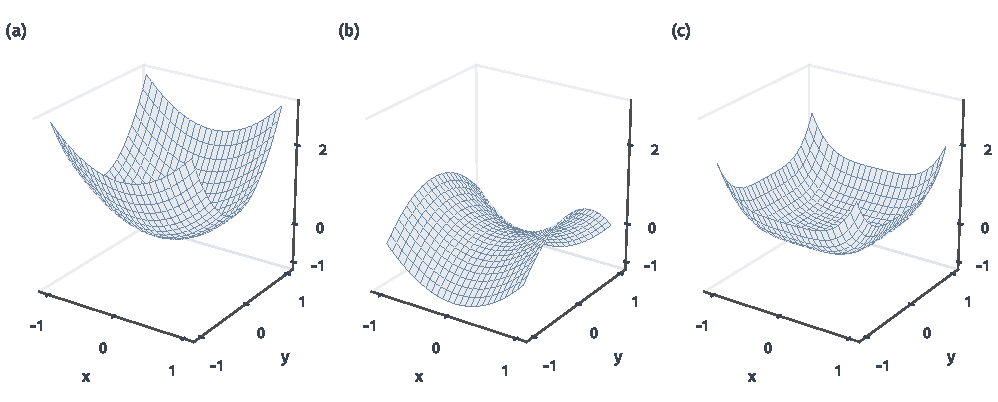
\includegraphics[width=169.0mm]{figures/00-shared/mathematical-preliminaries-upper/00-shared/matplotlib/chapter3-concept-processes/hessian-local-shapes.pdf}
 \caption{同一$[-1,1]^2$范围和纵轴尺度下，三面分别为$x^2+2y^2$、$x^2-y^2$、$x^4+y^4$。原点的Hessian依次为正定、不定、零矩阵；前两者给严格极小与鞍点，第三者虽严格极小却不能由正定判据推出。零Hessian也可能没有极值，例如前述$x^3$，故退化不是一种确定分类。}
 \label{fig:analysis-process-hessian-local-shapes}
\end{figure*}

\FloatBarrier

\section{多元向量值函数的微分}

前面每个输入只产生一个实数。现在固定$F:U\subseteq\mathbb R^d\to\mathbb R^m$，同一输入同时产生$m$个输出分量。例如极坐标映射$(r,\theta)\mapsto(r\cos\theta,r\sin\theta)$把两个参数变成平面上的点；神经网络的一层把输入向量变成另一个向量；参数曲线（$d=1$）与参数曲面（$d=2$、$m=3$）也是这种映射的特殊情况。
此时要问的是：输入稍作改变，输出点整体怎样移动。有限个输出可以逐分量检查，但每个分量的输入仍要整体扰动，不能以坐标切片代替各分量的全微分。

\subsection{向量值映射与Jacobian}

向量值函数由它的全部输出分量确定，因此按分量书写。
\begin{definition}[多元向量值函数]
\label{def:multivariable-vector-function}
映射$F:U\subseteq\mathbb R^d\to\mathbb R^m$称为多元向量值函数，写作$F=(F_1,\ldots,F_m)^\top$，其中每个$F_i:U\to\mathbb R$为多元标量函数。
\end{definition}
向量值函数的极限与连续性使用输出欧氏距离$\lVert F(\bm x)-\bm b\rVert_2$，即要求输出点整体接近$\bm b$。
对有限个输出，$F(\bm x)\to\bm b$等价于每个分量$F_i(\bm x)\to b_i$，$F$在一点连续也等价于每个$F_i$在该点连续，因为
\[
 \max_i|F_i(\bm x)-b_i|\leq\lVert F(\bm x)-\bm b\rVert_2
 \leq\sqrt m\max_i|F_i(\bm x)-b_i|.
\]
左侧不等式说明整体接近时每个分量都接近；右侧说明每个分量都接近到$\varepsilon/\sqrt m$以内时，整体误差小于$\varepsilon$。
这里分解的是输出分量，区别于只沿某些输入坐标检查的切片：每个分量$F_i$仍须在全部输入方向上联合趋近。

\paragraph{微分与Jacobian矩阵}

标量输出的全微分是到实数的线性映射，也称线性泛函；向量输出的全微分则要把输入扰动映射为$m$维输出扰动。
有限维线性映射由矩阵表示，矩阵的每一行记录一个输出分量的系数。
\begin{definition}[向量值函数的微分]
\label{def:multivariable-vector-differential}
设$U$开，$F:U\to\mathbb R^m$，$\bm a\in U$。若存在矩阵$\bm J_F(\bm a)\in\mathbb R^{m\times d}$，使
\begin{equation}
 F(\bm a+\bm h)=F(\bm a)+\bm J_F(\bm a)\bm h+o(\lVert\bm h\rVert_2),
\label{eq:analysis-jacobian-linearization}
\end{equation}
则称$F$在$\bm a$处可微，余项按输出欧氏范数理解。
其微分为$\mathrm dF_{\bm a}(\bm h)=\bm J_F(\bm a)\bm h$，其中$\bm J_F$称为\term{Jacobian矩阵}（Jacobian matrix），第$i,j$个元素为$\partial_jF_i$。
\end{definition}
向量值函数可微当且仅当每个输出分量$F_i$可微：正向可从向量余项取第$i$个分量，得到$F_i$的标量展开；反向则将有限个分量的$o(\lVert\bm h\rVert_2)$余项用欧氏范数合并，合并后仍是$o(\lVert\bm h\rVert_2)$。
因此Jacobian的第$i$行是标量分量梯度$\nabla F_i^\top$；$m=1$时Jacobian是梯度的转置，而不是梯度列向量本身。
$C^k$向量值函数指所有输出分量都属于$C^k$。

\paragraph{Jacobian矩阵的几何意义}
按列看Jacobian，第$j$列
\[
 \bm J_F(\bm a)\bm e_j=(\partial_jF_1,\ldots,\partial_jF_m)^\top
\]
表示：只把第$j$个输入增加一个很小的量$t$时，输出点大约沿这个向量移动$t$倍。一般扰动$\bm h=\sum_jh_j\bm e_j$的一阶效果就是这些列按$h_j$加权求和。
对$d=m=2$，这给出局部伸缩的图像：以$\bm a$为角、边长为$\varepsilon$的小正方形，由$\varepsilon\bm e_1,\varepsilon\bm e_2$张成，它的像近似是由$\varepsilon\bm J_F\bm e_1,\varepsilon\bm J_F\bm e_2$张成的平行四边形。行列式的绝对值是线性映射对面积的缩放倍数（第~\ref{sec:prelim-determinants}节），所以像的面积约为$|\det\bm J_F(\bm a)|\varepsilon^2$；行列式的符号说明局部是否翻转了定向。

极坐标映射给出这种局部伸缩的一个具体例子。
\begin{example}[极坐标映射的Jacobian矩阵]
\label{ex:multivariable-polar-jacobian}
考虑极坐标映射
\[
 P(r,\theta)=(r\cos\theta,r\sin\theta)^\top.
\]
逐个输出分量求偏导，得到
\[
\begin{gathered}
\bm J_P(r,\theta)=\begin{bmatrix}\cos\theta&-r\sin\theta\\ \sin\theta&r\cos\theta\end{bmatrix}\\
\det\bm J_P=r\cos^2\theta+r\sin^2\theta=r.
\end{gathered}
\]
第一列是单位径向向量：$r$增加$\mathrm dr$，点沿射线向外移动$\mathrm dr$。第二列长度为$r$、沿圆周切向：$\theta$增加$\mathrm d\theta$，点沿半径为$r$的圆移动约$r\,\mathrm d\theta$。因此参数平面中面积为$\mathrm dr\,\mathrm d\theta$的小矩形，变成面积约为$r\,\mathrm dr\,\mathrm d\theta$的小扇形块。
\end{example}

离原点越远，同样的角度增量扫过的弧越长，面积放大越多；第~\ref{sec:classical-change-variables}节的区域积分换元正是用这个倍数校正面积。

图~\ref{fig:analysis-process-jacobian-grid-cell}把一个非线性映射的线性近似画成小网格块的变化。图中$\det J_T(a)=1\times0.6-0.25\times0.3=0.525$，绿色小方块的像面积约为原面积的一半。
\begin{figure*}[!htbp]
 \centering
 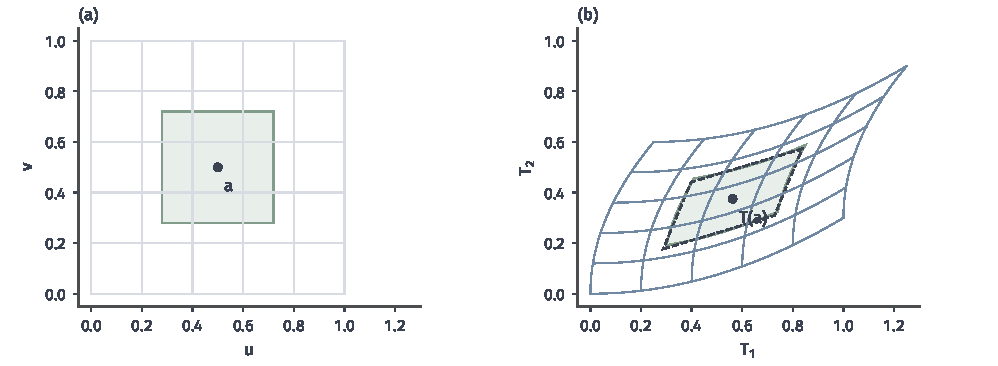
\includegraphics[width=169.0mm]{figures/00-shared/mathematical-preliminaries-upper/00-shared/matplotlib/chapter3-concept-processes/jacobian-grid-cell.pdf}
 \caption{取$T(u,v)=(u+v^2/4,\,0.6v+0.3u^2)$，$a=(0.5,0.5)$。(a) 输入网格及绿色小方块。(b) 非线性像为弯边块，黑虚线为$T(a)+J_T(a)(h,k)^\top$给出的平行四边形；$J_T(a)=\bigl[\begin{smallmatrix}1&0.25\\0.3&0.6\end{smallmatrix}\bigr]$。有限块不与线性像完全重合，缩小扰动后才由可微余项控制差异。}
 \label{fig:analysis-process-jacobian-grid-cell}
\end{figure*}

\paragraph{Jacobian矩阵的计算}
计算Jacobian矩阵时，每个输出先按标量函数求偏导，再按行排列；排好后可以核对输入、输出与矩阵形状是否一致。
例如$F(x,y)=(x^2+xy,y^2)^\top$的Jacobian为
\[
 \bm J_F(x,y)=\begin{bmatrix}2x+y&x\\0&2y\end{bmatrix}.
\]
在$(1,2)$处，它把扰动$(h,k)^\top$的一阶影响写成$(4h+k,4k)^\top$。两个输出分别占一行，两个输入分别占一列。

机器学习中一个常用的向量值映射，是把任意一组实数变成正数且总和为$1$的权重：先取指数，再除以共同的总和。
这就是$n$维\term{归一化指数映射}（softmax），分类模型常用它把各类别的得分变成概率。对正整数$n$和
$\bm{z}\in\mathbb{R}^n$，令
\[
 \begin{gathered}
s_i(\bm{z})
  =
  \frac{e^{z_i}}{\sum_{k=1}^n e^{z_k}}\\
i=1,\ldots,n.
 \end{gathered}
\]
记分母为$Z=\sum_k e^{z_k}$，它对$z_j$的偏导数为$e^{z_j}$。对分子$e^{z_i}$求偏导，$i=j$时得$e^{z_i}$，$i\neq j$时得$0$，记为$\mathbb{I}\{i=j\}e^{z_i}$。商法则给出
\[
  \frac{\partial s_i}{\partial z_j}
  =
  \frac{\mathbb{I}\{i=j\}e^{z_i}Z-e^{z_i}e^{z_j}}{Z^2}
  =
  s_i\bigl(\mathbb{I}\{i=j\}-s_j\bigr).
\]
因此整个Jacobian矩阵为
\begin{equation}
  \bm{J}_{\bm{s}}(\bm{z})
  =
  \operatorname{diag}(\bm{s})-\bm{s}\bm{s}^{\top}.
\label{eq:analysis-softmax-jacobian}
\end{equation}
这里$\operatorname{diag}(\bm s)$表示以$s_1,\ldots,s_n$为对角元、其他元素为零的对角矩阵。

当$n\geq2$时，对角项$s_i(1-s_i)$为正，描述提高$z_i$对自身分量的影响；非对角项$-s_is_j$为负，来自共同分母：提高一个得分会压低其余归一化分量。当$n=1$时输出恒为$1$，Jacobian为零。

每行元素之和为$s_i-s_i\sum_js_j=0$，这与给所有$z_i$同时加同一常数不改变输出相符：沿方向$(1,\ldots,1)^\top$的一阶变化为零。

在最简单的情形中，可以用数值核对式~\eqref{eq:analysis-softmax-jacobian}给出的线性近似。
\begin{example}[二维softmax的Jacobian矩阵]
\label{ex:multivariable-softmax-jacobian-check}
取$n=2$、$\bm z=\bm 0$，则$\bm s=(1/2,1/2)^\top$，由式~\eqref{eq:analysis-softmax-jacobian}，
\[
 \bm J_{\bm s}(\bm 0)
 =\begin{bmatrix}1/2&0\\0&1/2\end{bmatrix}-\begin{bmatrix}1/4&1/4\\1/4&1/4\end{bmatrix}
 =\begin{bmatrix}1/4&-1/4\\-1/4&1/4\end{bmatrix}.
\]
把$z_1$提高$0.1$，线性近似给出$\bm s$的增量约为
\[
 \bm J_{\bm s}(\bm 0)(0.1,0)^\top=(0.025,-0.025)^\top,
\]
即$s_1\approx0.525$、$s_2\approx0.475$。实际值为$s_1=e^{0.1}/(e^{0.1}+1)\approx0.52498$、$s_2\approx0.47502$。
\end{example}

线性近似与实际值只差约$2\times10^{-5}$，远小于输入改变量$0.1$；两个分量的增量一正一负、总和为零，与$s_1+s_2$恒为$1$相符。

\subsection{复合映射与导数的运算}
\label{sec:analysis-vector-chain-matrix-calculus}

运算法则以运算有定义为前提。输出形状相同的向量值函数可以相加、相减，任何向量值函数都可以数乘；复合则要求前一映射的输出落在后一映射的定义域内。
两个向量之间的乘法需要先指定含义（例如内积），本小节不讨论乘积法则。

\paragraph{和的微分}
若$F,H:U\to\mathbb R^m$在$\bm a$处可微，对每个输出分量分别使用标量的和法则，再把各分量的结果按行排回矩阵，得到
\[
 \bm J_{F+H}(\bm a)=\bm J_F(\bm a)+\bm J_H(\bm a).
\]
相加的输出形状以及两个Jacobian的形状必须分别一致。

\paragraph{差的微分}
在相同条件下，逐分量使用差法则，得到
\[
 \bm J_{F-H}(\bm a)=\bm J_F(\bm a)-\bm J_H(\bm a).
\]

\paragraph{数乘的微分}
对固定实数$c$，逐分量使用数乘法则，得到
\[
 \bm J_{cF}(\bm a)=c\bm J_F(\bm a).
\]

\paragraph{复合函数的链式法则}
复合映射$G\circ F$先用$F$把输入变成中间量，再用$G$把中间量变成输出。输入的小扰动$\bm h$先被$F$变成中间量的扰动，一阶上约为$\bm J_F\bm h$；这个扰动再被$G$变成输出扰动，一阶上约为$\bm J_G(\bm J_F\bm h)$。
因此复合微分按实际计算顺序组合，Jacobian的乘法次序由输入与输出维度决定。与一元情形一样，这项复合规则称为\term{链式法则}（chain rule）。
\begin{theorem}[向量值函数的链式法则]
\label{thm:multivariable-vector-chain-rule}
设$U\subseteq\mathbb R^d$、$V\subseteq\mathbb R^m$开，$F:U\to V$在$\bm a$处可微，$G:V\to\mathbb R^p$在$F(\bm a)$处可微，则$G\circ F$在$\bm a$处可微，且
\begin{equation}
 \bm J_{G\circ F}(\bm a)=\bm J_G(F(\bm a))\bm J_F(\bm a).
\label{eq:analysis-vector-chain-rule}
\end{equation}
\end{theorem}
\begin{proof}
记$\bm A=\bm J_F(\bm a)$、$\bm B=\bm J_G(F(\bm a))$。由$F$可微，中间量的增量为
\[
 \bm k=F(\bm a+\bm h)-F(\bm a)=\bm A\bm h+o(\lVert\bm h\rVert_2),
\]
故$\lVert\bm k\rVert_2\leq\lVert\bm A\bm h\rVert_2+o(\lVert\bm h\rVert_2)=O(\lVert\bm h\rVert_2)$：中间量的扰动与原扰动同阶。
代入$G$的一阶展开，
\[
 G(F(\bm a)+\bm k)-G(F(\bm a))=\bm B\bm k+o(\lVert\bm k\rVert_2)
 =\bm B\bm A\bm h+\bm B\,o(\lVert\bm h\rVert_2)+o(\lVert\bm k\rVert_2).
\]
右侧第二项中，矩阵$\bm B$至多把长度放大固定倍数，所以仍是$o(\lVert\bm h\rVert_2)$；第三项因$\lVert\bm k\rVert_2=O(\lVert\bm h\rVert_2)$也是$o(\lVert\bm h\rVert_2)$（$\bm k=\bm0$时外层余项为零）。
于是复合增量等于$\bm B\bm A\bm h$加上$o(\lVert\bm h\rVert_2)$，这正是复合函数的可微定义。
\end{proof}
式~\eqref{eq:analysis-vector-chain-rule}中的矩阵形状为$(p\times m)(m\times d)=p\times d$，反向相乘往往没有定义。
即使两个次序都有定义，矩阵乘法一般也不交换，不能按标量经验调换因子。
用局部伸缩的语言说：复合映射在一点附近的伸缩，等于两步伸缩依次作用；方阵情形下，行列式的乘法公式还给出面积缩放倍数相乘。

链式法则常用于这样的情形：先用向量值映射得到中间量，再把中间量变成一个标量，最后求这个标量对原输入的梯度。
\begin{example}[从中间向量求回复合目标的梯度]
\label{ex:analysis-chain-rule-calculation}
令
\[
 \begin{gathered}
F(x_1,x_2)=(x_1^2,x_1x_2,x_2)^\top\\
\ell(\bm y)=\frac12(y_1^2+y_2^2+y_3^2).
 \end{gathered}
\]
$F$从二维输入产生三维中间量，$\ell$再把三维中间量变成一个数，复合得到$L=\ell\circ F:\mathbb R^2\to\mathbb R$。
$\ell$的Jacobian是$1\times3$行向量$\nabla\ell(\bm y)^\top$，由链式法则，$L$的Jacobian为$\nabla\ell(F(\bm x))^\top\bm J_F(\bm x)$；转置后得到列向量梯度
\[
  \nabla L(\bm x)=\bm J_F(\bm x)^\top\nabla\ell\bigl(F(\bm x)\bigr).
\]
这里出现转置，是因为梯度按列向量书写，而链式法则中的$\ell$导数是行向量。本例中
\[
\begin{gathered}
\bm J_F=\begin{bmatrix}2x_1&0\\x_2&x_1\\0&1\end{bmatrix}\\
\nabla\ell(\bm y)=\bm y.
\end{gathered}
\]
在$\bm x=(1,2)^\top$处，$\bm y=(1,2,2)^\top$，链式法则给出
\[
  \nabla L(1,2)
  =\begin{bmatrix}2&2&0\\0&1&1\end{bmatrix}
    \begin{bmatrix}1\\2\\2\end{bmatrix}
  =\begin{bmatrix}6\\4\end{bmatrix}.
\]
也可以把复合函数直接展开为
$L(x_1,x_2)=\tfrac12(x_1^4+x_1^2x_2^2+x_2^2)$，求偏导得到
$\nabla L=(2x_1^3+x_1x_2^2,\,x_1^2x_2+x_2)^\top$，在同一点仍为$(6,4)^\top$。
矩阵形状$(2\times3)(3\times1)=2\times1$也核对了梯度传递的次序。
\end{example}

两种计算处理同一个目标；链式形式保留了中间映射，可以分别复用各层的导数。

\subsection{向量增量与导数范数估计}

标量函数的中值公式在线段上找到一个点，用那里的梯度精确表示增量。向量值函数不能照搬：各输出分量的一元中值点可能不同，没有一个共同位置代表整个向量增量。
例如$F(t)=(\cos t,\sin t)^\top$在$[0,2\pi]$上走完一整圈，$F(2\pi)-F(0)=\bm 0$，但速度$F'(t)=(-\sin t,\cos t)^\top$长度恒为$1$，不存在$\tau$使$F(2\pi)-F(0)=2\pi F'(\tau)$。
因此改为只控制增量的长度：用线性映射的最大放大倍数估计有限变化。

\paragraph{算子范数}

对标量函数，导数的绝对值说明输入的小变化被放大多少倍。对向量输出，同一矩阵在不同方向上放大的倍数可能不同，取其中最大的一个代替绝对值。
\begin{definition}[欧氏诱导算子范数]
\label{def:analysis-induced-operator-norm}
对矩阵
$\bm{A}\in\mathbb{R}^{s\times r}$，由欧氏范数\term{诱导的算子范数}
（induced operator norm）定义为
\[
  \lVert\bm{A}\rVert_{\mathrm{op}}
  =
  \sup_{\bm{h}\neq\bm{0}}
  \frac{\lVert\bm{A}\bm{h}\rVert_2}{\lVert\bm{h}\rVert_2}
  =
  \sup_{\lVert\bm{h}\rVert_2=1}\lVert\bm{A}\bm{h}\rVert_2.
\]
\end{definition}
算子范数是线性映射对向量长度的最大放大倍数，定义立即给出
$\lVert\bm{A}\bm{h}\rVert_2
\leq\lVert\bm{A}\rVert_{\mathrm{op}}\lVert\bm{h}\rVert_2$。
计算算子范数时，先给出对全部单位向量成立的上界，再找出达到上界的方向。
\begin{example}[对角矩阵的算子范数]
\label{ex:multivariable-diagonal-operator-norm}
令$\bm A=\operatorname{diag}(2,1)$，它把第一坐标放大两倍、第二坐标保持不变。对单位向量$\bm h$，
\[
 \lVert\bm A\bm h\rVert_2^2=4h_1^2+h_2^2\leq4(h_1^2+h_2^2)=4,
\]
且$\bm h=\bm e_1$时取等号，故$\lVert\bm A\rVert_{\mathrm{op}}=2$。
\end{example}

示例~\ref{ex:multivariable-diagonal-operator-norm}的最大放大由第一坐标方向达到。旋转矩阵不改变任何向量的长度，算子范数为$1$。

用算子范数控制增量长度后，就不再需要各分量共用一个中值点；所需条件是$G$在含整条线段的开集上连续可微。
\begin{theorem}[向量值函数的中值估计]
\label{thm:multivariable-vector-mean-value}
设$U\subseteq\mathbb R^r$开，$G:U\to\mathbb R^s$连续可微，且$[\bm y',\bm y]\subset U$，则
\begin{equation}
  \begin{aligned}
  \lVert G(\bm{y})-G(\bm{y}')\rVert_2
  &\leq
  \sup_{0\leq t\leq1}
  \left\lVert
    \bm{D}G\bigl(\bm{y}'+t(\bm{y}-\bm{y}')\bigr)
  \right\rVert_{\mathrm{op}}
  \lVert\bm{y}-\bm{y}'\rVert_2.
  \end{aligned}
\label{eq:analysis-operator-mean-value-bound}
\end{equation}
其中$\bm DG=\bm J_G$，即$G$的Jacobian矩阵。
\end{theorem}
\begin{proof}
思路是把向量增量投影到它自己的方向上，变成一个标量函数的增量，再对标量函数用中值定理。若$\bm u=G(\bm y)-G(\bm y')\neq\bm0$，
取单位向量$\bm v=\bm u/\lVert\bm u\rVert_2$，并沿线段定义标量函数
$\phi(t)=\bm v^\top G(\bm y'+t(\bm y-\bm y'))$。
由链式法则，$\phi'(t)=\bm v^\top\bm DG(\bm y'+t(\bm y-\bm y'))(\bm y-\bm y')$；中值定理给出某个$\tau\in(0,1)$，使
\[
 \lVert\bm u\rVert_2
 =\bm v^\top\bm u
 =\phi(1)-\phi(0)
 =\bm v^\top\bm DG(\bm y'+\tau(\bm y-\bm y'))(\bm y-\bm y').
\]
对右侧先用内积不等式并注意$\lVert\bm v\rVert_2=1$，再用算子范数的上界，便得到式~\eqref{eq:analysis-operator-mean-value-bound}；
$\bm u=\bm0$时该界直接成立。
\end{proof}
若定义域为凸开集，且Jacobian的算子范数在全域不超过同一个有限常数$L$，则由式~\eqref{eq:analysis-operator-mean-value-bound}，$G$以$L$为Lipschitz常数：任意两点的像之间的距离至多是原距离的$L$倍。在局部球上使用同样的界，就得到局部版本。
特别地，若Jacobian的算子范数在某个球内不超过一个常数$L<1$，映射就在球内严格缩小任意两点间的距离，称为压缩。第~\ref{sec:analysis-implicit-parameter-integral}节证明隐函数定理时，将用这一条件和几何级数的尾和控制迭代。

\section{矩阵函数的微分}

本小节的定义域$\mathcal U$均为全矩阵空间$\mathbb R^{m\times n}$中的开集，基点$\bm X\in\mathcal U$；因此全部充分小的同形扰动都允许使用。
机器学习中的参数常排成矩阵，例如线性层的权重或协方差矩阵，损失是它们的标量函数，求逆、相乘等运算又产生矩阵输出。原则上可以把矩阵拉直成长向量，再用前面的结论；但保留矩阵形状，能让乘法次序与迹的结构更清楚，结果也能直接写成矩阵表达式。

$m\times n$矩阵输入可以看成$mn$个实数坐标，$r\times s$矩阵输出可以看成$rs$个实数分量，因此可微性仍是“扰动的一阶变化由线性映射给出”；只是扰动用Frobenius范数度量，线性映射的输入与输出都保留矩阵形状。
第~\ref{sec:prelim-matrix-trace}节已定义Frobenius内积与范数，满足$\langle\bm A,\bm B\rangle_F=\operatorname{tr}(\bm A^\top\bm B)=\sum_{i,j}A_{i,j}B_{i,j}$，即把两个矩阵对应元素相乘再求和，也就是拉直后的向量内积。

\subsection{矩阵空间中的微分与梯度}
设$\Phi:\mathcal U\to\mathbb R^{r\times s}$。若存在矩阵空间之间的线性映射$\mathrm d\Phi_{\bm X}:\mathbb R^{m\times n}\to\mathbb R^{r\times s}$，使
\[
 \Phi(\bm X+\bm H)=\Phi(\bm X)+\mathrm d\Phi_{\bm X}(\bm H)+o(\lVert\bm H\rVert_F),
\]
余项按输出的Frobenius范数度量，则称$\Phi$在$\bm X$处可微，$\mathrm d\Phi_{\bm X}$为其微分。这就是向量值可微性按矩阵形状重排后的写法：Frobenius范数正是拉直后向量的欧氏范数。

计算时常写$\mathrm d\Phi=\mathrm d\Phi_{\bm X}(\mathrm d\bm X)$，用乘积法则展开后保留乘法次序。例如$\mathrm d(\bm A\bm X\bm B)=\bm A(\mathrm d\bm X)\bm B$，扰动夹在中间的位置不能移动。
又如$\Phi(\bm X)=\bm X^2=\bm X\bm X$，展开得$(\bm X+\bm H)(\bm X+\bm H)=\bm X^2+\bm H\bm X+\bm X\bm H+\bm H^2$。其中$\lVert\bm H^2\rVert_F\leq\lVert\bm H\rVert_F^2$是高阶项，故$\mathrm d(\bm X^2)=(\mathrm d\bm X)\bm X+\bm X(\mathrm d\bm X)$；只有$\bm X$与扰动交换时，才能写成$2\bm X\,\mathrm d\bm X$。

\paragraph{标量输出与矩阵梯度}
输出为标量（$r=s=1$）时，线性映射$\mathrm df_{\bm X}$可以用一个同形矩阵与扰动的Frobenius内积表示，这个矩阵就是梯度。这与向量情形$\mathrm df=\nabla f^\top\mathrm d\bm x$完全对应。
\begin{definition}[矩阵标量函数的梯度]
\label{def:multivariable-matrix-scalar-gradient}
设$f:\mathcal U\to\mathbb R$在$\bm X$处可微。唯一满足
\begin{equation}
 \mathrm df_{\bm X}(\bm H)=\langle\nabla_{\bm X}f,\bm H\rangle_F
 =\operatorname{tr}\bigl((\nabla_{\bm X}f)^\top\bm H\bigr)
\label{eq:analysis-matrix-gradient-definition}
\end{equation}
的同形矩阵$\nabla_{\bm X}f\in\mathbb R^{m\times n}$称为矩阵梯度。
\end{definition}
取只有第$(i,j)$个元素为$1$的扰动$\bm H$，右侧内积只剩$\nabla_{\bm X}f$的第$(i,j)$个元素，左侧是对$X_{i,j}$的偏导数。所以矩阵梯度的各元素就是对相应矩阵坐标的偏导数，唯一性也由此得到。与向量梯度一样，$\nabla_{\bm X}f$指出使$f$增加最快的扰动方向。

求梯度时，先用乘积法则展开微分，再利用迹的循环移位把扰动移到末端，写成$\operatorname{tr}(\bm G^\top\mathrm d\bm X)$的形式，便读出$\nabla_{\bm X}f=\bm G$。乘积形状相容时，
\[
 \begin{gathered}
\operatorname{tr}(\bm A\bm B)=\operatorname{tr}(\bm B\bm A)\\
\operatorname{tr}(\bm A\bm B\bm C)=\operatorname{tr}(\bm B\bm C\bm A).
 \end{gathered}
\]
这里循环移动的是整个因子，不能任意交换相邻矩阵。标量等于自己的迹，所以任何标量表达式都可以放进迹中再移位。
\begin{example}[双线性函数的矩阵梯度]
\label{ex:multivariable-bilinear-matrix-gradient}
对固定向量$\bm a\in\mathbb R^m$、$\bm b\in\mathbb R^n$，令$f(\bm W)=\bm a^\top\bm W\bm b$。它对$\bm W$线性，微分为$\mathrm df=\bm a^\top(\mathrm d\bm W)\bm b$。把这个标量写成迹并循环移位，
\[
 \mathrm df=\operatorname{tr}\bigl(\bm a^\top(\mathrm d\bm W)\bm b\bigr)=\operatorname{tr}\bigl(\bm b\bm a^\top\mathrm d\bm W\bigr)
 =\operatorname{tr}\bigl((\bm a\bm b^\top)^\top\mathrm d\bm W\bigr),
\]
于是$\nabla_{\bm W}f=\bm a\bm b^\top$。逐元素核对：$f=\sum_{k,l}a_kW_{k,l}b_l$，对$W_{i,j}$的偏导数是$a_ib_j$，正是$\bm a\bm b^\top$的第$(i,j)$个元素。
\end{example}

矩阵梯度的唯一性使用了全部矩阵方向。若把定义域限制在对称矩阵等子空间上，允许的扰动变少，满足式~\eqref{eq:analysis-matrix-gradient-definition}的矩阵不再唯一，还需另行说明所用的内积与允许方向。
矩阵输出时没有这样的单个梯度矩阵，只能保留线性映射$\mathrm d\Phi_{\bm X}$本身。以下依次计算迹、行列式与对数行列式这三个标量输出函数的微分，最后计算矩阵输出的逆矩阵。

\subsection{矩阵运算的微分法则}

加法、转置与迹是线性映射，其微分就是它们作用于扰动的结果。乘法则保留一阶的两种变化：若$A$、$B$同时变化，展开$(A+H)(B+K)$并舍去二阶项$HK$，得到
\[
 D(AB)[H,K]=HB+AK.
\]
Frobenius范数的乘积估计保证$\|HK\|_F\leq\|H\|_F\|K\|_F$，所以舍去项确实比联合扰动小一阶。复合运算按链式法则先计算内部扰动，再让外部微分作用于它；矩阵乘法次序始终保留。

线性迹函数已经符合定义，可以直接读出梯度。对固定的$\bm{A}\in\mathbb{R}^{m\times n}$，令$f(\bm{X})=\operatorname{tr}(\bm{A}^{\top}\bm{X})=\sum_{i,j}A_{i,j}X_{i,j}$。由于$f$线性，$f(\bm X+\bm H)-f(\bm X)=\operatorname{tr}(\bm A^\top\bm H)$，没有余项，微分已经是式~\eqref{eq:analysis-matrix-gradient-definition}的形式，所以
\begin{equation}
  \nabla_{\bm{X}}\operatorname{tr}(\bm{A}^{\top}\bm{X})
  =\bm{A}.
\label{eq:analysis-trace-linear-gradient}
\end{equation}
这与向量情形$\nabla_{\bm x}(\bm a^\top\bm x)=\bm a$对应，常用于从迹表达式中读出梯度。

\subsection{行列式的微分}
行列式把方阵映为一个实数，它的绝对值是线性映射对体积的缩放倍数（第~\ref{sec:prelim-determinants}节）。这里要问：矩阵稍作扰动，体积缩放倍数怎样变化。先在最简单的基点$\bm X=\bm I$处计算。
\begin{example}[单位矩阵附近行列式的一阶变化]
\label{ex:multivariable-determinant-near-identity}
取$\bm H=\operatorname{diag}(\varepsilon_1,\varepsilon_2)$，则
\[
 \det(\bm I+\bm H)=(1+\varepsilon_1)(1+\varepsilon_2)=1+\varepsilon_1+\varepsilon_2+\varepsilon_1\varepsilon_2,
\]
一阶变化是$\varepsilon_1+\varepsilon_2=\operatorname{tr}\bm H$。若扰动只在非对角位置，例如$\bm H=\begin{bmatrix}0&\varepsilon\\0&0\end{bmatrix}$，则$\det(\bm I+\bm H)=1$，面积不变，而$\operatorname{tr}\bm H=0$。
\end{example}

两个方向各拉长一点时，面积的相对增量一阶上是两个伸长率之和；剪切扰动不改变面积，迹也为零。两种情形中，一阶变化都等于扰动的迹。

一般情形设$\bm X\in\mathbb R^{d\times d}$可逆，以便用行列式的乘法公式把扰动从行列式中分离出来：
\[
 \det(\bm X+\bm H)=\det(\bm X)\det(\bm I+\bm X^{-1}\bm H).
\]
记$\bm B=\bm X^{-1}\bm H$。按第~\ref{sec:prelim-determinants}节的排列展开，$\det(\bm I+\bm B)$是$\bm B$的元素的多项式。恒等排列给出$\prod_i(1+B_{i,i})=1+\operatorname{tr}\bm B+(\text{二次及以上项})$；非恒等排列至少改变两个位置，每个改变的位置只能选到$\bm B$的非对角元，因而只贡献二次及以上项。于是
\[
 \det(\bm I+\bm B)=1+\operatorname{tr}\bm B+O(\lVert\bm B\rVert_F^2).
\]
又$\lVert\bm B\rVert_F\leq\lVert\bm X^{-1}\rVert_F\lVert\bm H\rVert_F$，所以余项对一切小扰动$\bm H$统一为$O(\lVert\bm H\rVert_F^2)$；这保证得到的是全微分，而不只是固定方向上的导数。代回$\bm B=\bm X^{-1}\bm H$，便得到Jacobi行列式公式的一阶形式
\[
 \mathrm{d}\det\bm{X}=\det(\bm{X})\operatorname{tr}(\bm{X}^{-1}\mathrm{d}\bm{X}).
\]
它说明有向体积缩放因子的相对变化$\mathrm d\det\bm X/\det\bm X$等于$\operatorname{tr}(\bm X^{-1}\mathrm d\bm X)$；$\bm X=\bm I$时回到示例~\ref{ex:multivariable-determinant-near-identity}中的$\operatorname{tr}\bm H$。

\subsection{对数行列式的微分}
实数对数还要求$\det\bm X>0$，满足这一条件的矩阵组成开集，对数在其上与行列式复合。对上面的微分应用标量对数的链式法则，$\mathrm d\log u=\mathrm du/u$，得到
\begin{equation}
\begin{gathered}
\mathrm{d}\log\det\bm{X}
  =
  \operatorname{tr}(\bm{X}^{-1}\mathrm{d}\bm{X})\\
\nabla_{\bm{X}}\log\det\bm{X}
  =
  \bm{X}^{-\top}.
\end{gathered}
\label{eq:analysis-logdet-gradient}
\end{equation}
第二式由$\operatorname{tr}(\bm X^{-1}\mathrm d\bm X)=\operatorname{tr}\bigl((\bm X^{-\top})^\top\mathrm d\bm X\bigr)$对照式~\eqref{eq:analysis-matrix-gradient-definition}读出。
若$\bm X$还对称，则$\bm{X}^{-\top}=\bm{X}^{-1}$；一般情形应保留转置。$1\times1$时它回到$(\log x)'=1/x$。
这些计算都先找出扰动的一阶项，再用迹内积读出梯度；乘积次序与行列式展开决定了哪些变形成立。

\subsection{求逆的微分}
求逆映射的输入与输出都是方阵，属于矩阵输出的情形。逆矩阵与行列式非零的关系已在第~\ref{sec:prelim-inverse-matrices}节及第~\ref{sec:prelim-determinants}节建立。
计算分两步：先确认可微，再对乘法恒等式取微分。
第~\ref{sec:prelim-determinants}节的代数余子式公式把逆矩阵的各元素写成多项式与$\det\bm X$之比。
因此在$\det\bm X\neq0$的开集内，每个元素都是分母非零的有理函数，连续可微，逆映射也连续可微。
确认可微性后，对恒等式$\bm{X}\bm{X}^{-1}=\bm{I}$两侧取微分，左侧用乘积法则，右侧是常矩阵，得到
\[
 (\mathrm{d}\bm{X})\bm{X}^{-1}+\bm{X}\,\mathrm{d}(\bm{X}^{-1})=\bm{0}.
\]
左乘$\bm{X}^{-1}$后得到
\begin{equation}
  \mathrm{d}(\bm{X}^{-1})
  =
  -\bm{X}^{-1}(\mathrm{d}\bm{X})\bm{X}^{-1}.
\label{eq:analysis-inverse-differential}
\end{equation}
$1\times1$时这就是$(1/x)'=-1/x^2$。两个$\bm{X}^{-1}$位于扰动两侧，不能合并成$-\bm{X}^{-2}\mathrm{d}\bm{X}$，因为$\mathrm{d}\bm{X}$未必与$\bm{X}^{-1}$交换。
取一个对角矩阵和一个非对角扰动，就能看出两种写法的差别。
\begin{example}[逆矩阵微分中的乘法次序]
\label{ex:analysis-noncommuting-inverse-differential}
取$\bm X=\operatorname{diag}(2,1)$，扰动方向
$\bm E=\begin{bmatrix}0&1\\1&0\end{bmatrix}$。由式~\eqref{eq:analysis-inverse-differential}，沿$\bm X+t\bm E$求逆矩阵在$t=0$处的导数为
\[
 -\bm X^{-1}\bm E\bm X^{-1}
 =\begin{bmatrix}0&-1/2\\-1/2&0\end{bmatrix}.
\]
若照搬标量规则而写成$-\bm X^{-2}\bm E$，会得到
$\begin{bmatrix}0&-1/4\\-1&0\end{bmatrix}$。
直接核对：$(\bm X+t\bm E)^{-1}=\frac1{2-t^2}\begin{bmatrix}1&-t\\-t&2\end{bmatrix}$，在$t=0$处对$t$求导，非对角元为$-1/2$，对角元导数为$0$，与第一种结果一致。
\end{example}

错误写法连对称性都丢失了。路径$\bm X+t\bm E$在$t=0$附近由对称可逆矩阵组成，它们的逆也对称，所以导数必须对称；这一结构检查能直接发现错误。矩阵变量沿给定方向微分时，夹在扰动两侧的逆矩阵不能随意移到同一侧。

\section{矩阵函数的一阶扰动分析}
\label{sec:multivariable-matrix-perturbation}

上一节求出了矩阵函数的微分。现在考虑另一个问题：已知矩阵$\bm A$和一个小扰动$\bm E$，怎样预测函数值的变化，预测的误差又有多大？微分给出一阶预测，但实际扰动总有有限大小，因此还需要检查近似的余项。

\subsection{微分与局部条件数}

设矩阵函数$\Phi$在$\bm A$处可微。对允许的扰动$\bm E$，其一阶变化为$\mathrm d\Phi_{\bm A}(\bm E)$。这是关于$\bm E$的线性映射；固定方向时，它描述该方向上的变化，并不代表其他方向有同样的响应。

若输入和输出空间分别选定范数，微分的算子范数
\[
 \lVert\mathrm d\Phi_{\bm A}\rVert
 =\sup_{\lVert\bm E\rVert=1}\lVert\mathrm d\Phi_{\bm A}(\bm E)\rVert
\]
给出单位扰动的一阶响应上界。如果只允许对称扰动等具有特定结构的变化，取上确界时也只能使用允许的方向。

输入和输出的尺度均非零时，可将这个上界乘以$\lVert\bm A\rVert/\lVert\Phi(\bm A)\rVert$，衡量相对扰动的一阶放大程度。它描述的是数学问题对输入变化的敏感性，不能单独说明某个求解算法是否稳定。

可微性只保证余项是$o(\lVert\bm E\rVert)$，不会自动给出某个有限扰动的数值误差界。若连接$\bm A$和$\bm A+\bm E$的线段位于定义域中，$\Phi$在该线段的一个开邻域内连续可微，并且微分在该线段上满足$\lVert\mathrm d\Phi_{\bm A+t\bm E}-\mathrm d\Phi_{\bm A}\rVert\leq Lt\lVert\bm E\rVert$，则沿线段应用一元微积分基本定理，得到
\[
 \left\lVert\Phi(\bm A+\bm E)-\Phi(\bm A)-\mathrm d\Phi_{\bm A}(\bm E)\right\rVert
 \leq\int_0^1 Lt\lVert\bm E\rVert^2\,\mathrm dt
 =\frac L2\lVert\bm E\rVert^2.
\]
这个二次上界依赖所给的邻域和常数$L$；下列例子分别核对这些条件。

\subsection{求逆的一阶近似}

取可逆方阵$\bm A$，由式~\eqref{eq:analysis-inverse-differential}，一阶预测为
\[
 (\bm A+\bm E)^{-1}\approx\bm A^{-1}-\bm A^{-1}\bm E\bm A^{-1}.
\]
使用向量范数诱导的矩阵范数（其单位矩阵范数为$1$，并满足乘积不等式），令$q=\lVert\bm A^{-1}\rVert\lVert\bm E\rVert<1$。此时$\bm I+\bm A^{-1}\bm E$可逆，其逆的范数不超过$1/(1-q)$。将$(\bm I+\bm A^{-1}\bm E)^{-1}$展开到一次项，并保留余项，得到
\[
 \left\lVert(\bm A+\bm E)^{-1}-\bm A^{-1}
 +\bm A^{-1}\bm E\bm A^{-1}\right\rVert
 \leq\frac{\lVert\bm A^{-1}\rVert^3\lVert\bm E\rVert^2}{1-q}.
\]
因此，扰动足够小时，预测误差按二次量缩小；当$q$接近$1$时，此界也提醒我们不能把一阶预测当成精确结果。线性方程中同时改变系数和右端项时，还需分别分析它们对解的影响。

\subsection{行列式的一阶近似}

在可逆矩阵$\bm A$处，行列式微分给出
\[
 \det(\bm A+\bm E)=\det\bm A\bigl(1+\operatorname{tr}(\bm A^{-1}\bm E)\bigr)+O(\lVert\bm E\rVert_F^2).
\]
其中迹是相对于原行列式的一阶变化；它随扰动方向而变。在固定有界邻域中，行列式作为矩阵元素的多项式，其二阶导数有界，所以可由沿$\bm A+t\bm E$的Taylor公式得到二次余项界。

奇异矩阵处仍可分析行列式的绝对变化，因为行列式是多项式；但此时$\det\bm A=0$，上式的相对变化和$\bm A^{-1}$都没有定义。行列式的数值小也不必然意味着求逆病态：例如$\bm A=\varepsilon\bm I$（$\varepsilon>0$）的行列式为$\varepsilon^d$，而它的二范数条件数仍为$1$。

\subsection{对数行列式的一阶近似}

设$\det\bm A>0$。取足够小的扰动，使整条线段都留在正行列式区域；由式~\eqref{eq:analysis-logdet-gradient}，有
\[
 \log\det(\bm A+\bm E)-\log\det\bm A
 =\operatorname{tr}(\bm A^{-1}\bm E)+o(\lVert\bm E\rVert_F).
\]
若原来的对数行列式接近零，以它为分母的相对误差不适合描述变化，此时应直接比较绝对变化及其尺度。

对称正定情形可以进一步给出具体余项界。设$\bm A$的最小特征值为$m>0$，$\bm E$对称且$\lVert\bm E\rVert_2<m$。对任意单位向量$\bm x$和$0\leq t\leq1$，
$\bm x^\top(\bm A+t\bm E)\bm x\geq m-\lVert\bm E\rVert_2>0$，因此整条线段保持正定。令$g(t)=\log\det(\bm A+t\bm E)$，则
\[
 g''(t)=-\operatorname{tr}\!\left((\bm A+t\bm E)^{-1}\bm E
 (\bm A+t\bm E)^{-1}\bm E\right).
\]
逆矩阵的二范数至多为$(m-\lVert\bm E\rVert_2)^{-1}$，由Frobenius内积和乘积估计，
$|g''(t)|\leq\lVert\bm E\rVert_F^2/(m-\lVert\bm E\rVert_2)^2$。一元Taylor公式于是给出
\[
 \left|\log\det(\bm A+\bm E)-\log\det\bm A
 -\operatorname{tr}(\bm A^{-1}\bm E)\right|
 \leq\frac{\lVert\bm E\rVert_F^2}{2(m-\lVert\bm E\rVert_2)^2}.
\]

例如$\bm A=\operatorname{diag}(2,1)$，$\bm E=\operatorname{diag}(0.1,0)$时，一阶预测为$0.05$，实际变化为$\log(1.05)\approx0.04879$。此时$m=1$，上述上界约为$0.00618$，大于实际误差约$0.00121$。这个界保证误差不超过多少，并不声称预测误差必然接近上界。


\section{隐函数与反函数}
\label{sec:analysis-implicit-parameter-integral}

前面对已给定的映射求微分；这里改变问题，先给定一组方程，再判断它是否在基点附近确定唯一的函数。
实际问题中，变量之间常由约束联系，而不是由显式公式给出：单位圆上的点满足$x^2+y^2=1$，物理系统的平衡状态满足力的平衡方程，模型训练的最优参数满足梯度为零。我们想知道，当一部分变量（参数）稍作改变时，其余变量（未知量）是否随之唯一地、光滑地改变，以及变化率是多少。
一般方程组用向量值映射表示。方程个数与待解变量个数相同时，关于待解变量的方阵Jacobian是否可逆，决定了能否在局部解出这些变量。

\subsection{隐函数的存在与微分}

显式函数直接给出输出，例如$y=\sqrt x$。关系$F(x,y)=0$则没有直接告诉我们给定$x$时$y$取什么值：可能有多个$y$满足方程，也可能一个都没有。

设$(a,b)$满足$F(a,b)=0$。若存在$a$附近的区间$I$、$b$附近的区间$J$和函数$\varphi:I\to J$，使得对$I\times J$中的点，$F(x,y)=0$成立恰好当$y=\varphi(x)$，就称方程在$(a,b)$附近确定了一个\term{隐函数}（implicit function）$y=\varphi(x)$。换句话说，只看$(a,b)$附近的小矩形，方程的解集恰是一个函数的图像。
隐函数研究的第一步是说明局部解分支存在且唯一，然后才对这条分支求导。

同一个方程在不同的点附近，可能确定隐函数，也可能不确定。
\begin{example}[单位圆附近的隐函数]
\label{ex:multivariable-implicit-circle}
考虑单位圆$x^2+y^2-1=0$。在$(0,1)$附近，解集是上半圆$y=\sqrt{1-x^2}$的一段；在$(0,-1)$附近则是下半圆$y=-\sqrt{1-x^2}$的一段，两处都确定了隐函数。
但在$(1,0)$附近，每个略小于$1$的$x$对应上下两个解，略大于$1$的$x$没有解；无论矩形多小，解集都不是关于$x$的函数图像。此处圆的切线是竖直的。
\end{example}

解集分成几支时，还要指定从哪一个解出发。
\begin{example}[方程$y^2=x$的两支解]
\label{ex:multivariable-implicit-parabola-branches}
方程$y^2-x=0$在$x>0$时有正、负两支解$y=\pm\sqrt x$。固定其中一个非零解，例如$(1,1)$，可以在它附近选出唯一的正支。
但在$(0,0)$处两支相交，负$x$侧又没有实数解，因此不存在定义在含$0$的开区间上的解函数。
\end{example}

两个例子中不能局部解出$y$的点，都满足$\partial F/\partial y=2y=0$：单位圆在$(1,0)$处如此，$y^2-x$在$(0,0)$处也如此。这正是定理~\ref{thm:analysis-implicit-function}所要求的可逆性失效的地方。因此，局部选解既要指定起始解，也要核对关于待解变量的导数。

图~\ref{fig:vol1-add-implicit-branches}说明“局部唯一”怎样排除另一支解。在$(1,1)$附近只保留正支即可；在原点处，两支相交且负$x$没有实数解，不能用同样的方式局部选出可微的解。
\begin{figure}[!htb]
  \centering
  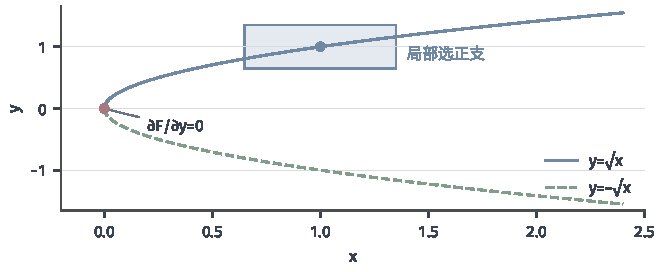
\includegraphics[width=112mm]{figures/00-shared/mathematical-preliminaries-upper/00-shared/matplotlib/mathematical-language-combinatorics-analysis-optimization-comprehension-additions/implicit-branches.pdf}
  \caption{方程$F(x,y)=y^2-x=0$的两支实数解。浅蓝矩形围住$(1,1)$，在该矩形内每个允许的$x$只有正支解，且$F_y=2y\neq0$；红点处$F_y=0$，两支相交。两支解满足同一方程，选定起始解与邻域才确定隐函数分支。}
  \label{fig:vol1-add-implicit-branches}
\end{figure}
\FloatBarrier


\paragraph{存在、唯一性与微分}

为什么条件是关于待解变量的导数可逆？先看线性方程。

设$\bm x\in\mathbb R^p$为参数、$\bm y\in\mathbb R^m$为未知量，$\bm P\in\mathbb R^{m\times p}$、$\bm Q\in\mathbb R^{m\times m}$固定，方程$\bm P\bm x+\bm Q\bm y=\bm 0$有$m$个方程、$m$个未知量。当$\bm Q$可逆时，对每个$\bm x$都有唯一解$\bm y=-\bm Q^{-1}\bm P\bm x$；$\bm Q$不可逆时，解要么不存在，要么不唯一。

对非线性方程$F(\bm x,\bm y)=\bm 0$，可微性说明它在基点附近近似于线性方程
\[
 \bm D_{\bm x}F(\bm a,\bm b)(\bm x-\bm a)+\bm D_{\bm y}F(\bm a,\bm b)(\bm y-\bm b)\approx\bm 0,
\]
其中$\bm D_{\bm x}F$、$\bm D_{\bm y}F$分别是只对$\bm x$、只对$\bm y$的坐标求偏导排成的Jacobian块。隐函数定理断言：只要线性近似中$\bm Q=\bm D_{\bm y}F$可逆，非线性方程在局部也像线性方程一样有唯一解，而且解的导数就是线性解的系数$-\bm Q^{-1}\bm P$。

隐函数定理给出的是充分条件：先保证局部解存在且唯一，再保证解随参数连续可微。
可逆性只要求待解变量对应的方阵Jacobian可逆，并不要求整个带参数映射的Jacobian是方阵。
\begin{theorem}[隐函数定理]
\label{thm:analysis-implicit-function}
设$F:\mathbb{R}^p\times\mathbb{R}^m\to\mathbb{R}^m$在$(\bm{a},\bm{b})$的某个开邻域内连续可微，$F(\bm{a},\bm{b})=\bm{0}$，并且关于待解变量的Jacobian矩阵
\[
 \bm{D}_{\bm{y}}F(\bm{a},\bm{b})\in\mathbb{R}^{m\times m}
\]
可逆。则存在$\bm{a}$与$\bm{b}$的邻域$U,V$，以及唯一的连续可微函数
$\varphi:U\to V$，使$\varphi(\bm{a})=\bm{b}$，并且对所有
$(\bm{x},\bm{y})\in U\times V$都有
\[
  F(\bm{x},\bm{y})=\bm{0}
  \quad\Longleftrightarrow\quad
  \bm{y}=\varphi(\bm{x}).
\]
其Jacobian矩阵满足
\begin{equation}
  \bm{D}\varphi(\bm{x})
  =
  -
  \bigl[\bm{D}_{\bm{y}}F(\bm{x},\varphi(\bm{x}))\bigr]^{-1}
  \bm{D}_{\bm{x}}F(\bm{x},\varphi(\bm{x})).
\label{eq:analysis-implicit-derivative}
\end{equation}
\end{theorem}
若已知$\varphi$存在且可微，导数公式可以直接由链式法则得到：对恒等式$F(\bm x,\varphi(\bm x))=\bm 0$求导，得$\bm D_{\bm x}F+\bm D_{\bm y}F\,\bm D\varphi=\bm 0$，再左乘$(\bm D_{\bm y}F)^{-1}$。定理真正困难的部分是$\varphi$的存在、唯一与可微，形式求导不能替代这些步骤。

证明的思路是把解方程改写为反复修正的迭代。一元时，固定$x$，从$y_0=b$出发，用$y_{n+1}=y_n-F(x,y_n)/F_y(a,b)$不断修正：若$F(x,y_n)>0$且$F_y(a,b)>0$，就把$y$调小一点。这类似Newton法，只是斜率固定用基点处的值。若每次修正都使误差按固定比例缩小，迭代就收敛到唯一解。
证明分别检查三件事：修正映射是压缩；它不把点送出所考察的球；所得解随参数可微。
\begin{proof}
为证明定理~\ref{thm:analysis-implicit-function}的存在性，先把方程改写为局部压缩迭代。记
\[
 \begin{gathered}
\bm{A}=\bm{D}_{\bm{y}}F(\bm{a},\bm{b})\\
T_{\bm{x}}(\bm{y})=\bm{y}-\bm{A}^{-1}F(\bm{x},\bm{y}).
 \end{gathered}
\]
因为$\bm A^{-1}$可逆，$F(\bm{x},\bm{y})=\bm{0}$当且仅当$T_{\bm{x}}(\bm{y})=\bm{y}$，即$\bm y$是更新后保持不变的点，称为不动点。并且
\[
 \bm{D}_{\bm{y}}T_{\bm{x}}(\bm{y})=\bm{I}-\bm{A}^{-1}\bm{D}_{\bm{y}}F(\bm{x},\bm{y}),
\]
它在$(\bm{a},\bm{b})$处为零。由$F$的导数连续，这个矩阵的元素在基点附近都很小；又由Cauchy--Schwarz不等式，算子范数不超过Frobenius范数。因而可以选择闭球$B=\{\bm{y}:\lVert\bm{y}-\bm{b}\rVert_2\leq r\}$和$\bm{a}$的邻域$U$，使
\begin{equation}
  \sup_{\bm{x}\in U,\,\bm{y}\in B}
  \left\lVert
    \bm{D}_{\bm{y}}T_{\bm{x}}(\bm{y})
  \right\rVert_{\mathrm{op}}
  \leq q<1.
\label{eq:analysis-ift-uniform-contraction}
\end{equation}
沿$\bm{y}$方向使用式~\eqref{eq:analysis-operator-mean-value-bound}（球是凸集，球内线段不离开球）可知，每个
$T_{\bm{x}}$都把$B$内任意两点之间的距离缩小到原来的至多$q$倍。

还必须核对自映射，即$T_{\bm x}$不把$B$中的点送出$B$；否则迭代可能离开压缩成立的范围。因为$T_{\bm{a}}(\bm{b})=\bm{b}$且$T_{\bm{x}}(\bm{b})$关于$\bm{x}$连续，可进一步缩小$U$，使
\[
 \lVert T_{\bm{x}}(\bm{b})-\bm{b}\rVert_2\leq\frac{1-q}{2}r.
\]
于是对$\bm{y}\in B$，先用三角不等式拆开，再用压缩性，
\[
 \begin{aligned}
  \lVert T_{\bm{x}}(\bm{y})-\bm{b}\rVert_2
  &\leq
  \lVert T_{\bm{x}}(\bm{y})-T_{\bm{x}}(\bm{b})\rVert_2+\lVert T_{\bm{x}}(\bm{b})-\bm{b}\rVert_2\\
  &\leq
  q\lVert\bm{y}-\bm{b}\rVert_2+\frac{1-q}{2}r
  \leq
  \frac{1+q}{2}r
  <r.
 \end{aligned}
\]
所以$T_{\bm{x}}(B)$包含在$B$的内部$V$中。
固定$\bm x\in U$，从$\bm y_0=\bm b$出发，令$\bm y_{n+1}=T_{\bm x}(\bm y_n)$。
所有迭代项都留在$B$内，每一步的压缩使相邻差满足
$\lVert\bm y_{n+1}-\bm y_n\rVert_2\leq q\lVert\bm y_n-\bm y_{n-1}\rVert_2\leq\cdots\leq q^n\lVert\bm y_1-\bm y_0\rVert_2$。
增大$q$仍保留这个上界，因而可设$0<q<1$。对$m>n$，几何和给出
\[
 \lVert\bm y_m-\bm y_n\rVert_2
 \leq\sum_{j=n}^{m-1}\lVert\bm y_{j+1}-\bm y_j\rVert_2
 \leq\frac{q^n}{1-q}\lVert\bm y_1-\bm y_0\rVert_2\longrightarrow0.
\]
每个坐标都是实柯西列，所以该序列在有限维欧氏空间中收敛；闭性使极限仍在$B$内。
$T_{\bm x}$连续，在$\bm y_{n+1}=T_{\bm x}(\bm y_n)$中令$n\to\infty$，可得极限$\varphi(\bm x)$满足
$T_{\bm x}(\varphi(\bm x))=\varphi(\bm x)$，而$T_{\bm x}(B)\subset V$使它属于$V$。
若另有不动点$\bm z\in B$，则
$\lVert\bm z-\varphi(\bm x)\rVert_2=\lVert T_{\bm x}(\bm z)-T_{\bm x}(\varphi(\bm x))\rVert_2\leq q\lVert\bm z-\varphi(\bm x)\rVert_2$，
由$q<1$只能有$\bm z=\varphi(\bm x)$，所以这个不动点唯一。若
$(\bm{x},\bm{y})\in U\times V$且$F(\bm{x},\bm{y})=\bm{0}$，则$\bm{y}\in B$也是
$T_{\bm{x}}$的不动点，唯一性迫使$\bm{y}=\varphi(\bm{x})$。这证明了定理所述的局部
存在与零点集合的逐点唯一性。

还需说明所得解随参数连续可微。先证$\varphi$局部Lipschitz连续，即它不会随参数剧烈变化。把$U$进一步缩小为开球，并使
$\overline U\times B$包含在原定义域内；这个集合闭且有界，$T_{\bm x}(\bm y)$关于$\bm x$的导数$-\bm A^{-1}\bm D_{\bm x}F$各分量连续，
故有统一范数上界$L$。对$\bm x,\bm x'\in U$，
两点间的线段仍在$U$内，式~\eqref{eq:analysis-operator-mean-value-bound}
可用于$T_{\bm x}(\bm y)$的参数变化。利用两个不动点关系$\varphi(\bm x)=T_{\bm x}(\varphi(\bm x))$、$\varphi(\bm x')=T_{\bm x'}(\varphi(\bm x'))$，把差拆成“改变$\bm y$”与“改变$\bm x$”两步：
\[
 \begin{aligned}
 \lVert\varphi(\bm{x})-\varphi(\bm{x}')\rVert_2
 &\leq\lVert T_{\bm x}(\varphi(\bm x))-T_{\bm x}(\varphi(\bm x'))\rVert_2\\
 &\quad+\lVert T_{\bm x}(\varphi(\bm x'))-T_{\bm x'}(\varphi(\bm x'))\rVert_2\\
 &\leq q\lVert\varphi(\bm{x})-\varphi(\bm{x}')\rVert_2+L\lVert\bm{x}-\bm{x}'\rVert_2,
 \end{aligned}
\]
移项得到$\lVert\varphi(\bm x)-\varphi(\bm x')\rVert_2
\leq L\lVert\bm x-\bm x'\rVert_2/(1-q)$，
故$\varphi$局部Lipschitz连续。

再证可微。令$\bm{h}\to\bm{0}$并记$\bm{k}=\varphi(\bm{x}+\bm{h})-\varphi(\bm{x})$，前述界给出$\lVert\bm{k}\rVert_2=O(\lVert\bm{h}\rVert_2)$。两点都在解集上，所以
\[
 F(\bm{x}+\bm{h},\varphi(\bm{x})+\bm{k})-F(\bm{x},\varphi(\bm{x}))=\bm{0}.
\]
对左侧作联合扰动$(\bm h,\bm k)$的一阶展开，得到
\[
 \bm{D}_{\bm{x}}F\,\bm{h}+\bm{D}_{\bm{y}}F\,\bm{k}+o(\lVert\bm{h}\rVert_2)=\bm{0}.
\]
展开中的Jacobian均在$(\bm x,\varphi(\bm x))$处取值，联合扰动的余项
$o(\lVert(\bm h,\bm k)\rVert_2)$因$\lVert\bm k\rVert_2=O(\lVert\bm h\rVert_2)$
成为$o(\lVert\bm h\rVert_2)$。
基点的$\det\bm A\neq0$，行列式又是矩阵元素的连续函数，
所以邻域足够小时$\bm D_{\bm y}F$仍可逆。左乘它的逆，得到
\[
 \bm{k}=-(\bm{D}_{\bm{y}}F)^{-1}\bm{D}_{\bm{x}}F\,\bm{h}+o(\lVert\bm{h}\rVert_2).
\]
这证明$\varphi$可微并给出式~\eqref{eq:analysis-implicit-derivative}；右侧各Jacobian矩阵及矩阵求逆都连续，又保证$\bm{D}\varphi$连续。至此，隐函数定理中的存在、局部唯一与导数公式都已得到证明。
\end{proof}

\paragraph{隐函数的导数}

定理的证明已同时建立解分支的存在、唯一性、可微性及式~\eqref{eq:analysis-implicit-derivative}。计算时只需在选定分支上代入两个Jacobian。用示例~\ref{ex:multivariable-implicit-parabola-branches}和示例~\ref{ex:multivariable-implicit-circle}的方程，可以核对不同分支各自的变化率。

\begin{example}[隐函数分支的导数]
设$F(x,y)=y^2-x$，在$(1,1)$处有$F=0$、$F_y=2\neq0$。
隐函数定理保证$(1,1)$附近的解可以唯一写成$y=\varphi(x)$，且
\[
 \begin{gathered}
\varphi'(x)=-\frac{F_x(x,\varphi(x))}{F_y(x,\varphi(x))}
 =\frac1{2\varphi(x)}\\
\varphi'(1)=\frac12.
 \end{gathered}
\]
直接选正支$\varphi(x)=\sqrt x$，求导同样得到$1/(2\sqrt x)$。
若在$(1,-1)$附近选负支，导数则为$-1/2$。

对单位圆$x^2+y^2=1$上半圆的一点$(x_0,y_0)$（$y_0>0$），同一公式给出$\varphi'(x_0)=-x_0/y_0$，不必先解出$y=\sqrt{1-x^2}$。
\end{example}

起始解不同，所追踪的函数也不同，导数公式要在选定分支上取值。单位圆的导数$-x_0/y_0$在$y_0\to0$时趋于无穷，与$(1,0)$处的竖直切线相符，也与示例~\ref{ex:multivariable-implicit-circle}中$(1,0)$附近不能把$y$解成$x$的函数相一致。

\subsection{特征值与特征向量的局部微分}

隐函数定理也能研究矩阵变化时的特征方向。设实对称矩阵$\bm S_0\in\mathbb R^{d\times d}$有一个简单特征值$\lambda_0$，对应单位特征向量$\bm v_0$。简单表示这个特征值的代数重数为$1$；对实对称矩阵，这等价于其特征空间是一维的。即使规定向量长度为$1$，$\bm v_0$和$-\bm v_0$仍代表同一方向；为了在局部选定一支，我们要求附近的向量$\bm v$满足$\bm v_0^\top\bm v>0$。

把对称矩阵$\bm S$作为参数，选取其上三角元素作为独立坐标，便可把对称矩阵空间视为有限维欧氏空间。把向量$\bm v$和标量$\lambda$作为未知量。特征方程与单位长度条件合起来写成
\[
 F(\bm S,\bm v,\lambda)=
 \begin{pmatrix}\bm S\bm v-\lambda\bm v\\ (\bm v^\top\bm v-1)/2\end{pmatrix}=\bm0.
\]
在$(\bm S_0,\bm v_0,\lambda_0)$处，关于$(\bm v,\lambda)$的导数作用于$(\bm h,\eta)$，其矩阵为
\[
 \begin{pmatrix}\bm S_0-\lambda_0\bm I&-\bm v_0\\
 \bm v_0^\top&0\end{pmatrix}.
\]
若该矩阵把$(\bm h,\eta)$映为零，先用$\bm v_0^\top$左乘第一行，利用对称性及$\bm S_0\bm v_0=\lambda_0\bm v_0$得到$\eta=0$；第二行给出$\bm v_0^\top\bm h=0$。此时$\bm h$既属于$\lambda_0$的特征空间，又与$\bm v_0$正交。由于特征值简单，只能有$\bm h=\bm0$。因此这个方阵可逆，隐函数定理保证在$\bm S_0$附近存在可微的特征值和单位特征向量分支；上述内积为正的条件固定了局部符号。

对称扰动方向$\bm E$使特征值与特征向量分别产生一阶变化$\dot\lambda$和$\dot{\bm v}$。对特征方程与归一化条件求微分，并在基点取值，得到
\[
 \begin{gathered}
(\bm S_0-\lambda_0\bm I)\dot{\bm v}
 =-(\bm E-\dot\lambda\bm I)\bm v_0\\
\bm v_0^\top\dot{\bm v}=0.
 \end{gathered}
\]
用$\bm v_0^\top$左乘第一式，便得到$\dot\lambda=\bm v_0^\top\bm E\bm v_0$。把它代回后，右侧与$\bm v_0$正交；由于$\lambda_0$简单，$\bm S_0-\lambda_0\bm I$限制在$\bm v_0$的正交补上可逆，因此第二式选出了唯一的$\dot{\bm v}$。

这里的结论依赖所选特征值简单。重特征值使上述关于未知量的导数失去可逆性，因此不能直接用这个构造；这并不意味着每一条特征值分支都不可微。研究重根附近时，可以改为考察相应特征子空间，而不是强行指定其中某一个特征向量。


\subsection{局部反函数与坐标变换}

另一个常见问题是反求输入：已知映射$G$的输出$\bm y$，能否唯一确定产生它的输入$\bm x$，并且$\bm x$随$\bm y$光滑变化。例如由直角坐标$(x,y)$反求极坐标$(r,\theta)$。
线性映射$\bm y=\bm M\bm x$可逆当且仅当方阵$\bm M$可逆；非线性映射在一点附近近似于它的Jacobian，所以可以期待：Jacobian可逆时，映射在局部可逆。
把$G(\bm x)-\bm y=\bm 0$看成以输出为参数、输入为待解变量的一组方程，就能使用隐函数定理。
定理只给出两个邻域之间的逆映射，不断言$G$在整个定义域上单射。
\begin{theorem}[局部反函数定理]
\label{thm:multivariable-inverse-function}
设$U\subseteq\mathbb R^d$开，$G:U\to\mathbb R^d$连续可微，$\bm a\in U$，且$\bm J_G(\bm a)$可逆。
则存在$\bm a$的开邻域$U_0$与$G(\bm a)$的开邻域$V_0$，使$G:U_0\to V_0$为双射，逆映射连续可微，并满足
\[
 \bm J_{G^{-1}}(G(\bm x))=[\bm J_G(\bm x)]^{-1}
 \qquad(\bm x\in U_0).
\]
\end{theorem}
\begin{proof}
以输出$\bm y$为参数、原输入$\bm x$为待解变量，令$H(\bm y,\bm x)=G(\bm x)-\bm y$。
在$(G(\bm a),\bm a)$处，关于$\bm x$的Jacobian就是可逆的$\bm J_G(\bm a)$。隐函数定理给出开邻域$V_0$、$W$以及$C^1$映射$\varphi:V_0\to W$，使
\[
 G(\bm x)=\bm y\quad\Longleftrightarrow\quad\bm x=\varphi(\bm y)
 \qquad(\bm y\in V_0,\ \bm x\in W).
\]
将$W$缩小并重新选取$V_0$，可使$W\subset U$且$\bm J_G$在$W$内均可逆。
令$U_0=W\cap G^{-1}(V_0)$，它因$G$连续而为包含$\bm a$的开集。
每个$\bm y\in V_0$都有$G(\varphi(\bm y))=\bm y$，故$\varphi(\bm y)\in U_0$；反之，每个$\bm x\in U_0$都由上述唯一性满足$\varphi(G(\bm x))=\bm x$。
因此$G:U_0\to V_0$为双射，逆就是$C^1$映射$\varphi$。
对$G(\varphi(\bm y))=\bm y$使用链式法则，得到$\bm J_G(\varphi(\bm y))\bm J_\varphi(\bm y)=\bm I$，左乘逆矩阵便得到所述公式。
\end{proof}
公式说明，逆映射的局部伸缩恰好抵消原映射的局部伸缩。极坐标映射可以具体说明这一点。
\begin{example}[极坐标的局部反函数]
\label{ex:multivariable-polar-local-inverse}
对$P(r,\theta)=(r\cos\theta,r\sin\theta)^\top$，示例~\ref{ex:multivariable-polar-jacobian}算得$\det\bm J_P=r$，所以在$r>0$的每一点附近，都可以从$(x,y)$唯一、光滑地反求$(r,\theta)$。在$(r,\theta)=(2,\pi/2)$，即平面上的点$(0,2)$处，
\[
\begin{gathered}
\bm J_P=\begin{bmatrix}0&-2\\1&0\end{bmatrix}\\
\bm J_{P^{-1}}(0,2)=\bm J_P^{-1}=\begin{bmatrix}0&1\\-1/2&0\end{bmatrix}.
\end{gathered}
\]
第一行说明$\mathrm dr=\mathrm dy$：在正上方的点，向上移动直接增大半径。第二行说明$\mathrm d\theta=-\mathrm dx/2$：向左移动使角度增大，且因为半径为$2$，角度变化只有水平位移的一半。
\end{example}

在原点$r=0$处，Jacobian行列式为零，所有$\theta$都映到同一点，确实无法反求$\theta$；这正是定理条件不满足的地方。

\paragraph{局部可逆与整体单射}

Jacobian处处可逆仍不保证映射在整个定义域上单射。
\begin{example}[Jacobian处处可逆而不单射]
\label{ex:multivariable-local-not-global-inverse}
考虑映射
\[
\begin{gathered}
g(u,v)=(e^u\cos v,e^u\sin v)^\top\\
(u,v)\in\mathbb R^2.
\end{gathered}
\]
它的Jacobian矩阵为
\[
\begin{gathered}
\bm J_g(u,v)=\begin{bmatrix}e^u\cos v&-e^u\sin v\\ e^u\sin v&e^u\cos v\end{bmatrix}\\
\det\bm J_g=e^{2u}>0,
\end{gathered}
\]
处处可逆。但$(u,v)$与$(u,v+2\pi)$给出同一输出，$g$不是单射。
\end{example}

这个$g$就是半径取$e^u$的极坐标映射：在每一点附近可以反求，整个平面上的输入却绕着原点重复覆盖输出。

另一方面，存在连续逆也不保证逆可微：一元函数$x\mapsto x^3$全局单射，其逆$y\mapsto y^{1/3}$在$0$处没有有限导数；这正对应$x^3$在$0$处导数为零，定理条件不满足。使用局部反函数定理时，需要逐项检查邻域、可微性和Jacobian的可逆性。

\FloatBarrier


\FloatBarrier
\section{本章小结}
\label{sec:multivariable-differentiation-summary}

多元极限要求所有趋近方式给出同一结果，只检查坐标轴或直线还不够。可微要求所有小扰动共用一个线性近似；偏导数或各方向导数存在，并不单独保证可微。梯度给出标量函数的一阶变化，Jacobian矩阵记录向量值映射的微分，Hessian矩阵描述二阶变化，并在相应条件下帮助判断驻点附近的形状。

矩阵微分保留输入和输出的形状，也保留矩阵乘法次序。对求逆、行列式和对数行列式，微分给出一阶扰动预测；要控制有限扰动的误差，还须核对定义域和余项界。隐函数与反函数定理说明，在选定基点且相关Jacobian可逆时，方程或映射在邻域中确定可微分支；这种局部结论不能替代全局唯一性。
